\documentclass[onecolumn]{report}

\usepackage{color}
\usepackage{amsmath}
\usepackage{ulem}


%\usepackage{apjfonts}
\usepackage{txfonts} % looks nice

\bibliographystyle{apj}

\definecolor{brown}{rgb}{0.42,0.24,0.07}
\definecolor{green}{rgb}{0.0,0.6,0.00}
\definecolor{purple}{rgb}{0.7,0.0,0.7}
\definecolor{black}{rgb}{0.0,0.0,0.0}
\def\red#1{\textcolor{red}{#1}}
\def\cyan#1{\textcolor{cyan}{#1}}
\def\blue#1{\textcolor{blue}{#1}}
\def\green#1{\textcolor{green}{#1}}
\def\brown#1{\textcolor{brown}{#1}}
\def\purple#1{\textcolor{purple}{#1}}

\newcommand\cut[1]{\red{\sout{#1}}}

%%% Useful commands
\newcommand{\alex}[1]{\green{{#1}}}
\newcommand{\marc}[1]{\brown{{#1}}}
\newcommand{\wlad}[1]{\purple{{#1}}}
\newcommand{\areli}[1]{\cyan{{#1}}}
\newcommand{\comm}[1]{\blue{{#1}}} %for updates for referee comments
\newcommand{\beq}{\begin{equation}}
\newcommand{\eeq}{\end{equation}}
\newcommand{\ben}{\begin{eqnarray*}}
\newcommand{\een}{\end{eqnarray*}}

% Variables:
\newcommand{\Sigmagas}{\ensuremath{\varSigma_\mathrm{g}}}
\newcommand{\Sigmadust}{\ensuremath{\varSigma_\mathrm{d}}}
\newcommand{\Sigmagasref}{\ensuremath{\varSigma_\mathrm{g,0}}}
\newcommand{\OmegaK}{\ensuremath{\varOmega_\mathrm{K}}}
\newcommand{\Omegagas}{\ensuremath{\varOmega}}
\newcommand{\Omegaref}{\ensuremath{\varOmega_\mathrm{0}}}
\newcommand{\rhogas}{\ensuremath{\rho_\mathrm{g}}}
\newcommand{\rhodust}{\ensuremath{\rho_\mathrm{d}}}
\newcommand{\rhopmat}{\ensuremath{\rho_\mathrm{mat}}}
\newcommand{\epsdtog}{\ensuremath{\epsilon_\mathrm{d/g}}}
\newcommand{\phieffi}{\varPhi_{\mathrm{eff}}}
\newcommand{\nsuper}{N}
\newcommand{\nsub}{n}
\newcommand{\tauf}{\tau_\mathrm{f}}
\newcommand{\taucool}{\tau_\mathrm{cool}}
\newcommand{\zetape}{\zeta_\mathrm{pe,0}}
\newcommand{\Gammape}{\varGamma_\mathrm{pe}}
\newcommand{\Tref}{T_\mathrm{0}} % reference temperature profile
\newcommand{\alphaSS}{\ensuremath{\alpha}} % Shakura-Sunyaev alpha
\newcommand{\alphaSSref}{\ensuremath{\alpha}} % Shakura-Sunyaev alpha at reference radius
\newcommand{\alphaSB}{\alpha_\mathrm{SB}} % surface brightness slope
\newcommand{\alphaOD}{\alpha_\mathrm{OD}} % optical depth slope
\newcommand{\tauOD}{\ensuremath{\tau_\mathrm{OD}}} % optical depth
\newcommand{\tauODchar}{\ensuremath{\breve{\tau}_\mathrm{OD}}} % optical depth
\newcommand{\tauchar}{\ensuremath{\tilde{\tau}}} % optical depth
\newcommand{\betaPR}{\ensuremath{\beta_\mathrm{PR}}} % Poynting-Robertson beta
\newcommand{\betaPRref}{\ensuremath{\beta_\mathrm{PR,0}}} % Poynting-Robertson beta
\newcommand{\betai}{\ensuremath{\beta_\mathrm{PR}}} % Poynting-Robertson beta
\newcommand{\rBR}{\ensuremath{r_\mathrm{BR}}} % reference radius (birth ring)
\newcommand{\tcol}{t_{\rm col}}
\newcommand{\treside}{t_{\rm reside}}
\newcommand{\ThetaPE}{\ensuremath{\Theta}}
\newcommand{\St}{\ensuremath{\mathrm{St}}}
\newcommand{\mmm}{\ensuremath{\mu}}
\newcommand{\Mstar}{\ensuremath{M_\star}}
\newcommand{\Lstar}{\ensuremath{L_\star}}
\newcommand{\dragcoef}{\ensuremath{C_D}}
\newcommand{\e}{\ensuremath{e}}
\newcommand{\grainradius}{\ensuremath{a}}
\newcommand{\cs}{\ensuremath{c_s}}
\newcommand{\vv}{\ensuremath{\v{v}}}
% Units:
\newcommand{\Msun}{\ensuremath{M_\odot}}
\newcommand{\Mearth}{\ensuremath{M_\oplus}}
\newcommand{\Mdust}{\ensuremath{M_\mathrm{dust}}}
\newcommand{\AU}{\ensuremath{\mathrm{AU}}}
\newcommand{\micrometer}{\ensuremath{\muup\mathrm{m}}}
\newcommand{\Lsun}{\ensuremath{L_\odot}}
\newcommand{\cm}{\ensuremath{\mathrm{cm}}}
\newcommand{\gram}{\ensuremath{\mathrm{g}}}
\newcommand{\gcmtwo}{\ensuremath{\gram~\cm^{-2}}}
% Operators:
\newcommand{\deriv}[2]{\frac{d{#1}}{d{#2}}}
\newcommand{\pderiv}[2]{\frac{\partial{#1}}{\partial{#2}}}
\newcommand{\ptderiv}[1]{\frac{\partial{#1}}{\partial{t}}}
\renewcommand{\v}[1]{{\boldsymbol{#1}}}
\newcommand{\aderiv}[1]{\frac{D{#1}}{D t}}
\newcommand{\del}{\v{\nabla}}
\newcommand{\grad}{\del}
\newcommand{\Div}{\del\cdot}

\newcommand{\Figure}[1]{Figure~\ref{#1}}
\newcommand{\Fig}[1]{Fig.~\ref{#1}}
\newcommand{\fig}[1]{\Fig{#1}}
\newcommand{\Figs}[2]{Figs.~\ref{#1} and \ref{#2}}
\newcommand{\Eq}[1]{Eq. (\ref{#1})}
\newcommand{\Eqs}[2]{Eqs. (\ref{#1}) and~(\ref{#2})}
\newcommand{\Eqss}[2]{Eqs. (\ref{#1})--(\ref{#2})}
\newcommand{\eq}[1]{\Eq{#1}}
\newcommand{\eqs}[2]{\Eqs{#1}{#2}}
\newcommand{\eqss}[2]{\Eqss{#1}{#2}}
\newcommand{\eqp}[1]{(Eq. \ref{#1})}
\newcommand{\eqt}[1]{Eq. \ref{#1}}
\newcommand{\advec}{\left(\v{u}\cdot\del\right)}
\newcommand{\Table}[1]{Table~\ref{#1}}
\newcommand{\sect}[1]{Sect.~\ref{#1}}


\newcommand{\beqn}{\begin{eqnarray}}
\newcommand{\eeqn}{\end{eqnarray}}
\newcommand{\cv}{c_{_{V}}}
\newcommand{\cp}{c_p}
\newcommand{\taut}{\tau_{_T}}
\newcommand{\xtimes}[2]{${#1}\times 10^{#2}$}


\usepackage{multirow}

\usepackage[export]{adjustbox}
\usepackage{bm}
\usepackage{gensymb}
\usepackage{color}

\def\cyan#1{\textcolor{cyan}{#1}}
\def\green#1{\textcolor{green}{#1}}

\usepackage{indentfirst}
\setlength{\parindent}{0.5cm}
\usepackage{graphicx}
\graphicspath{{figures/}}
\usepackage{subcaption}
\usepackage{float}
\usepackage{color}
\usepackage{setspace}
\usepackage{amsmath}
\usepackage{sectsty}

\usepackage{geometry}
 \geometry{
 left=1.5in,
 top=1in,
 right=1in,
 bottom=1in,
 }

\pagenumbering{roman}

\newcommand{\startsquarepar}{%
    \par\begingroup \parfillskip 0pt \relax}
\newcommand{\stopsquarepar}{%
    \par\endgroup}

\newcommand{\epsi}{\varepsilon}

\renewcommand{\contentsname}{\normalfont \large \vspace{-60pt} \hspace{160pt} Table of Contents}
\renewcommand{\listfigurename}{\normalfont \large \vspace{-60pt}\hspace{173pt} List of Figures}
\renewcommand{\bibname}{\normalfont \large References}

\usepackage{tocloft}
\renewcommand\cftchapfont{\normalfont \large}
\renewcommand\cftchappagefont{\normalfont \large}
\renewcommand\cftloftitlefont{\normalfont \large}

\def\bibindent{1.5em}
\makeatletter
\let\old@biblabel\@biblabel
\def\@biblabel#1{\old@biblabel{#1}\kern\bibindent}
\let\old@bibitem\bibitem
\def\bibitem#1{\old@bibitem{#1}\leavevmode\kern-\bibindent}
\renewcommand\@biblabel[1]{}
\makeatother

\allsectionsfont{\centering \normalfont \large}

\newsavebox\foobox
\def\slantvalue{0}
\newcommand{\slantboxengine}[2][\slantvalue]{\mbox{%
        \sbox{\foobox}{#2}%
        \hskip\wd\foobox
        \pdfsave
        \pdfsetmatrix{1 0 #1 1}%
        \llap{\usebox{\foobox}}%
        \pdfrestore
}}
\newcommand\slantbox[2][\slantvalue]{%
  \edef\slantvalue{#1}\expandafter\slantboxhelpA#2 \relax\relax}
\def\slantboxhelpA#1 #2\relax{%
  \slantboxengine{#1}%
  \ifx\relax#2\relax\else\ \slantboxhelpA#2\relax\fi
}

\setcounter{secnumdepth}{3}
\setcounter{tocdepth}{3}
\renewcommand{\thesubsubsection}{\arabic{chapter}.\arabic{section}.\arabic{subsection}.\alph{subsubsection}}

\makeatletter
\def\@makechapterhead#1{%
  \vspace*{-30\p@}%
  {\parindent \z@ \center \normalfont
    \ifnum \c@secnumdepth >\m@ne
        \large\normalfont \@chapapp\space \thechapter
        \par\nobreak
        \vskip 10\p@
    \fi
    \interlinepenalty\@M
    \large \normalfont #1\par\nobreak
    \vskip 10\p@
  }}

\def\@makeschapterhead#1{%
  %\vspace*{50\p@}%
  {\parindent \z@ \center
    \normalfont
    \interlinepenalty\@M
    \Huge \bfseries  #1\par\nobreak
    \vskip 20\p@
  }}
\makeatother

\usepackage{titletoc}%
\titlecontents{chapter}% <section-type>
  [0pt]% <left>
  {\normalfont}% <above-code>
  {\chaptername\ \thecontentslabel: }% <numbered-entry-format>
  {}% <numberless-entry-format>
  {\hfill\contentspage}% <filler-page-format>

%%%%%%%%%%%%%%%%%%%%%%%%%%%%%%%%%%%%%%%%%%%%%%%%%%%   ~~~!!~!!!~! end Alex stuff

\mathchardef\mathhyphen="2D

%\begin{document}

%%%%%%%%%%%%%%%%%%%%%%%%%%%%%%%%%%%%%%%%%%%%%%%%%%%   ~~~!!~!!!~! start Alex stuff

\begin{document}

\thispagestyle{empty}

\begin{center}
\large

CALIFORNIA STATE UNIVERSITY, NORTHRIDGE \\~\\~\\~\\~\\~\\ ~\\~\\~\\~\\

Disentangling the Effect of Planets from Photoeletric Instability In Gas-Rich Optically Thin Dusty Disks \\~\\~\\~\\~\\~\\~\\~\\~\\~\\

A thesis submitted in partial fulfillment of the requirements \\~\\

for the degree of Master of Science in Physics \\~\\~\\~\\~\\~\\~\\~\\

By \\~\\ Areli Castrejon


\vfill

May 2018

\end{center}

\normalfont
\newpage
\addcontentsline{toc}{section}{\hspace{-19pt} Signature Page}

The thesis of Areli Castrejon is approved: \\~\\~\\~\\~\\~\\~\\~\\


------------------------------------------------------------------ \hfill ---------------------------

Dr. Farisa Morales \hfill Date \hspace{75pt} \\~\\~\\~\\~\\~\\

------------------------------------------------------------------ \hfill ---------------------------

Dr. Luca Ricci \hfill Date \hspace{75pt} \\~\\~\\~\\~\\~\\

------------------------------------------------------------------ \hfill ---------------------------

Dr. Adam Burgasser \hfill Date \hspace{75pt} \\~\\~\\~\\~\\~\\

------------------------------------------------------------------ \hfill ---------------------------

Dr. Geoffrey Bryden \hfill Date \hspace{75pt} \\~\\~\\~\\~\\~\\

------------------------------------------------------------------ \hfill ---------------------------

Dr. Wladimir Lyra, Chair \hfill Date \hspace{75pt}

\vfill
\begin{center}
California State University, Northridge
\end{center}

\doublespacing

\begin{center}
\newpage
\section*{\normalfont Acknowledgements}
\addcontentsline{toc}{section}{\hspace{-19pt} Acknowledgements}
\thispagestyle{plain}
\end{center}

ACKNOWLEDGEMENTS GO HERE


\newpage
\begin{center}
\section*{\normalfont Dedication}
\addcontentsline{toc}{section}{\hspace{-19pt} Dedication}
\thispagestyle{plain}
\end{center}

DEDICATIONS GO HERE

\newpage
\singlespacing

\tableofcontents

\clearpage
\addcontentsline{toc}{section}{\hspace{-19pt} List of Figures}
\listoffigures

\clearpage
\begin{center}
\addcontentsline{toc}{section}{\hspace{-19pt} Abstract}
\section*{Abstract}
\thispagestyle{plain}

\doublespacing
\large

Disentangling Planets from Photoelectric Instability In Gas-Rich Optically Thin Dusty Disks  \\~\\~\\~\\

By

Areli Castrejon

Master of Science in Physics \\~\\~\\~\\

\end{center}

\doublespacing
\large

Structures found in circumstellar disks, such as gaps and rings are attributed to planets. Yet, this causation thus far has been difficult to show unequivocally, as other disk processes may also produce these features. In particular, a photoelectric instability (PEI) has been proposed as a parallel cause for structures. The instability operates in gas-rich optically thin disks, and generate non-trivial structures, including some predicted by planet-disk interactions. We examine the question of how to disentangle planetary effects on disk structure from those of the photoelectric instability. We use the Pencil Code to perform two-dimensional global hydriodynamic models of the dynamics of gas and dust in a non-magnetized thin disk, with and without planetary perturbers. Photoelectric heating is modeled with an equation of state where the pressure if proportional to the dust surface density (short thermal time approximation). The drag force on grains and its backreaction on the gas are included. Starting without the effect of the photoelectric heating, we find that dust-gas interactions alter the shape of the planetary gap from the dust-free case when the local dust-to-gas ratio $\varepsilon$ approaches unity. This result is valid also for primordial disksm because as the dust drifts inwards, the dust front becomes a sharp transition and, the backreaction triggers the Rossby wave instability. When photoelectric heating is included, we find that the photoelectric instability obscures structures induced by planets unless the plaent's mass is sufficiently large to carve a noticeable gap. More specifically, the instability generates ars and rings of regular spacing: a planet is discernable when it carves a dust gap wider than the wavelength of the instability

\chapter{Introduction and Background} %\label{chap:introduction-and-background}

\pagenumbering{arabic}
\setcounter{page}{1}

\section{Circumstellar Disks: Introduction}

One of the oldest questions that all civilizations, ancient and modern alike, have tried to answer is the origin of humankind. We want to know where we came from, and ultimately where that will lead us. We cannot answer this question without first asking how our planed formed. Since the first time telescopes were pointed at the sky, we have inched closer  to answering the riddle behind planet formation, and the creation of our own.

The widely accepted model for the creation of star systems, and consequentially, planet formation is the nebular hypothesis. Clouds of interstellar gas remain in equilibrium, until they grow too massive and collapse under their own gravitational influence. The rotational kinetic eergy is conserved, and as a star forms in the center, the cloud flattens out to form a disk. This becomes the protostellar disk around the newly-formed star.

In the disk, there are large quantities of dust and gas that could lead to planet formation, much in the same way that the star and the protoplanetary disk formed. In this case, planets can be formed by two mechanisms. The two mechanisms are gravitational instability and direct accretion.

Whenever we have a have region in the disk that becomes cool or develops a large surface density, it can incite gravtitational instabilities. This can produce: local and global spiral waves \textbf{citations needed}, self-gravitating turbulence \textbf{citations needed}, and fragmentation into clumps and other substructures \textbf{citations needed}, the latter of which could potentially lead to form giant planets.

In the accretion model, we have dust grains in the $\mu m$ range that through interactions, grow into larger size particulates. They grow into pebbles and through gravitational instabilities they grow into planetesimals, creating planets.

\section{Structures in Disks} %\label{sec:observation}

Disks have been theorized to exist, due to the nebular hypothesis that was mentioned earlier. However, due to constraints on our telescopes, we had not been able to discern them.

Recent observations from ALMA and VLT have shown us more disks than we have seen in the past. The increase in angular resolution has made it so that we are able to see disks more clearly. The disks we have observed now show structures that are found to be non-trivial.

One of these structures are rings. Rings have been found around HL Tau, between 20 and 100 AU. In TW Hydra, we have also found ring structures, that are not well defined, between 2 to 40 AU.

In tandem with rings, we also find gaps, which are areas devoid of gas and dust \textbf{The following disks show gap structures + citations}.

The observations have also shown azimuthal symmetries. These symmetries are crescent shaped emissions. Two disks that show this structure are HD 142527 and LkH$\alpha$ \textbf{references}. 

The question now becomes, what can we attribute these structures to? The first conclusion that comes to mind is the presence of planet. The planet would clear out its orbit, causing the gaps that we see in the observation, while also explaning the rings. Planets can also incite the spirals in disks, if the planet is massive enough to drag gas along with it during its orbital motion.

\section{The Photoelectric Instability}

While that is valid conclusion, it overlooks one aspect that is of importance in optically-thin disks. Disks are usually classified as gas-rich or gas-free. There are some disks in this regime that have amounts of gas that are comparable to the amount of dust. In this case, the dust and the gas can become dynamically significant to the same degree. When this happens we propose a new mechanism that can give rise to the structures that are usually attributed to planets. This mechanism is called the photoelectric instability.

The photoelectric instability happens when high-energy photons from the star strip electrons from the dust grains. The electrons ejected are superthermal. They have a higher energy than surrounding gas, and through collisions they impart their kinetic energy to the gas. The gas becomes heated due to the collisions, creating a pressure bump. Now that the gas has a pressure bump, the inner and outer edges of the pressure bump are out of equilibrium with the rest of the disk. The inner part feel a positive pressure gradient (towards the star), which decreases their effective gravity, causing them to rotate faster than the Keplerian velocity. Gas parcels on the outer part of the pressure bump feel a negative pressure gradient, which increases their effective gravity, causing them move slower than the Keplerian velocity. The motions of the dust are changed due to this. In the inner part, the gas moves faster than the dust, which makes the dust feel a tailwind, pushing it into a higher orbit. In the outer part, the gas moves slower than the dust, causing it (dust) to feel a headwind, making it move into a lower orbit. This creates a snowball effect that causes more dust to concentrate at the location of the pressure bump. This runaway effect of capturing more dust, which leads to more heating, is the mechanism behind the creation of the arcs, gaps, and rings that we see in optically-thin circumstellar disks.

An important aside, the photoelectric instability only applies for a certain subset of disk. It applies to late-stage transitions disks and debris disks. This application of the model to this small subset is drawn from the fact, that only in these two case, are the dust and gas present in equal amounts. In young disks, such as protoplanetary and primordial disk \textbf{?}, gas is present at a much higher ratio than dust. The gas dominates the motions of the disk and the dust is no dynamically significant. Transitions disks are middle-aged \textbf{?} disks that are characterized by a large cavity in the inner region of the disk. Debris disks are \textbf{Big ol' ?}. However they can contain significant amounts of gas if \textbf{? (finish this)}

\section{The Model}

\subsection{Run Parameters}

The simulations are performed on a uniform cylindrical grid (coordnates $r$, $\phi$), with a resolution of ($N_r$, $N_{\phi}$) = (528, 528), and a linear domain $L_r$=[0.4,2.5] and full 2$\pi$ coverage in azimuth(\textbf{get this explained too}). The 200,000 dust grains are modeled as Lagrangian superparticles scattered uniformly across the disk. The star and the planet orbit around a shared center of mass in circular orbits. The self-gravity of the disk is ignored. We ran simulations with three different planet masses. The mass ratios of the planets with respect to the host star are $q = 10^{-3}, 10^{-4}, 10^{-5}$. For each planet, we simulated five dust-to-gas ratios from $10^{-4}$ to 1, spaced logarithmically. The highest growth rate for the PEI are in the regime between $\epsi=10^{-2}$ \& $\epsi=1$.

The parameters of the simulations we ran are in Table.~\ref{table:allmodels}. In order to investigate the effect of the photoelectric instability we ran 36 simulations. We used to planets, a Jupiter and Neptune analog. For each planet, we varied 3 disk temperatures (T = 5, 20, 80K), 2 dust-to-gas ratios ($\epsi=10^{-1},1$), and 3 different cases for gap carving in the disk. The three cases are: a planet with no photoelectric instability, a disk with instability on its own, and a combined case with an embedded planet and the instability.

\begin{table}
  \caption[]{Parameter space explored in our simulations: $h$ is the
    disk scale height of the disk, $\varepsilon$ is the initial
    dust-to-gas ratio, and $q$ is the planet-to-star mass ratio.
    The letter identifier in the first column is shown in the upper
    left corner of each plot in this paper, for easier referral.}
  \label{table:allmodels}
  \begin{center}
    \begin{tabular}{lcc c} \hline \hline
      \multirow{2}{*} \sc{Run} & h  & $\varepsilon$ & $q$ \\
      \multicolumn{4}{c}{\multirow{2}{*}{Fiducial runs with no dust}}\\\\\hline
      i  & 0.05 & $0$ & $10^{-3}$\\
      ii & 0.05 & $0$ & $10^{-4}$\\\hline
      \multicolumn{4}{c}{\multirow{2}{*}{Runs with a single planet.}}\\\\\hline
      A & 0.05 & $10^{-1}$ & $10^{-3}$\\
      B & 0.05 & $10^{-1}$ & $10^{-4}$\\
      F & 0.05 & $1$       & $10^{-3}$\\
      G & 0.05 & $1$       & $10^{-4}$\\
      K & 0.1  & $1$       & $10^{-3}$\\
      L & 0.1  & $1$       & $10^{-4}$\\
      P & 0.2  & $1$       & $10^{-3}$\\
      Q & 0.2  & $1$       & $10^{-4}$\\
      AA & 0.05 & $10^{-4}$ & $10^{-3}$\\
      AB & 0.05 & $10^{-4}$ & $10^{-4}$\\
      AC & 0.05 & $10^{-3}$ & $10^{-3}$\\
      AD & 0.05 & $10^{-3}$ & $10^{-4}$\\
      AE & 0.05 & $10^{-2}$ & $10^{-3}$\\
      AF & 0.05 & $10^{-2}$ & $10^{-4}$\\\hline
      \multicolumn{4}{c}{\multirow{2}{*}{Runs with photoelectric instability.}}\\\\\hline
      C & 0.05 & $10^{-1}$ & 0\\
      H & 0.05 & $1$       & 0\\
      M & 0.1  & $1$       & 0\\
      R & 0.2  & $1$       & 0\\\hline
      \multicolumn{4}{c}{\multirow{2}{*}{Runs with a planet and instability.}}\\\\\hline
      D & 0.05 & $10^{-1}$ & $10^{-3}$\\
      E & 0.05 & $10^{-1}$ & $10^{-4}$\\
      I & 0.05 & $1$       & $10^{-3}$\\
      J & 0.05 & $1$       & $10^{-4}$\\
      N & 0.1  & $1$       & $10^{-3}$\\
      O & 0.1  & $1$       & $10^{-4}$\\
      S & 0.2  & $1$       & $10^{-3}$\\
      T & 0.2  & $1$       & $10^{-4}$\\\hline
      \multicolumn{4}{c}{\multirow{2}{*}{Runs with no gas backreaction.}}\\\\\hline
      BA & 0.05 & $10^{-1}$ & 0\\
      BB & 0.05 & $10^{-2}$ & 0\\\hline
    \end{tabular}
  \end{center}
\end{table}

\newpage

\subsection{The Equations} %\label{subsec:basic-structure}

In order to solve the steady-state solution of the gas in a disk we need to solve the hydrodynamic equations and the equation for the gravitational potential.

For a protoplanetary disk, two simplifications are made. We usually assume that the mass of the disk is much smaller than the mass of the star, such that $M_{star} >> M_{disk}$. 

In our models, we assume that we are dealing with a disk where the radius is much larger than the thickness, such that $r > h$. This is called the thin-disk approximation, since the vertical structure becomes superfluous, and we can model the disk in two dimensions instead of 3. We include gas and dust in our simulations. Dust is treated as Lagrangian particles and the gas is evolved on a Eulerian grid. We solve the different equations for the dynamics which are as follows:

\beqn
\pderiv{\varSigma_g}{t} &=& -\advec{\varSigma_g} -\varSigma_g \Div{\v{u}}, \label{eq:continuity} \\ %+ f_D(\varSigma\_g)\\
\pderiv{\v{u}}{t} &=& -\advec{\v{u}} -\frac{1}{\varSigma_g}\grad{P} - \grad{\varPhi} - \frac{\varSigma_d}{\varSigma_g}\frac{\left(\v{u}-\v{v}\right)}{\tauf}, \label{eq:euler}\\
\pderiv{S}{t} &=& -\advec{S} -\frac{c_V}{T}\frac{\left(T-T_p\right)}{\taut}, \label{eq:entropy}\\
\varPhi &=& \sum_i^n\frac{GM_i}{\sqrt{{R_i}^2 + {b_i}^2}}, \label{eq:potential}\\
P &=& \rho {c_s}^2/\gamma, \label{eq:eos}\\
\frac{d\v{x}}{dt} &=& \v{v}, \label{eq:position-dust}\\
\frac{d\v{v}}{dt} &=& -\grad{\varPhi} - \frac{\left(\v{v}-\v{u}\right)}{\tauf} \label{eq:momentum-dust},
\eeqn

Here $\varSigma_g$ and $\varSigma_d$ are the vertically integrated gas density and bulk density of the dust respectively; $\textbf{u}$ stands for the velocity of the gas parcels; $P$ is the vertically integrated pressure, $\varPhi$ is the gravitational potential, and $\v{v}$ is the velocity of the dust grains. The gravitational potential includes contributions from the star and embedded planets, treated as massive particles with a N-body evolution dynamically integrated with the hydrodynamics evolution. In \eq{eq:potential}, $G$ is he gravitational constant, $M_i$ is the mass of particle $i$, located at $\v{r}_{p_i}$. The quantity $b_i$ is the distance over which the gravity field of the particles $i$, is softened to prevent singularities. In \eq{eq:entropy}, $S$ is the gas entropy given by:

\beq
S = \cv\left[ \ln\left(\frac{P}{P_0}\right) - \gamma \ln\left(\frac{\varSigma_g}{\varSigma_{g0}}\right)\right]
\eeq

where $\cv$ is the specigic heat at constant volume, $\gamma=\cp / \cv$ is the adiabatic index, and $\cp$ is the specific heat at constant pressure. $P_0$ and $\Sigma_{g0}$ are reference pressure and gas density values, respectively. In \eq{eq:entropy} $T$ stands for the gas temperature:

\beq
T = \frac{c_s^2}{\cp\left(\gamma-1\right)}
\eeq

where $c_s$ is the sound speed; $\tau_T$ is the thermal coupling times between gas and dust. The quantity $T_p$ is a simple prescription for the gas temperature set by the photoelectric heating. \textbf{KlahrLin05}

\beq
T_p = T_0\left(\frac{\varSigma_d}{\varSigma_{g0}}\right)^\beta \label{eq:reftemperature}\\
\eeq

where $T_0$ is a reference temperature and we keep $\beta=1$. In the Lagrangian dust equations, $\v{v}_p$ is the velocity of a dust grain, and $\v{x}_p$ is their position. The last term in \eq{eq:euler} is the drag force, by which the dust and gas interact dynamically. The last term in \eq{eq:momentum-dust} is the backreaction of the drag force. We use:

\beq
\tauf = \tauf{_0}\left(\frac{\varOmega_0}{\varOmega}\right)
\eeq

and keep $\tauf{_0}\varOmega_0 = 1$.  The operator

\beq
\frac{D}{Dt} = \ptderiv{} + \v{u} \cdot \del
\eeq

\noindent represents the advective derivative. Given that the goal of this work is to exaine the competing roles of the PEI and gravitational perturbation by a planet, we ignored the effects of the radiation pressure. Because the termal time is expected to be very loew, we use the instantaneous thermal coupling approximation. \textbf{LyraKuchner13}. That means that instaed of solving the energy equation, we equate $T=T_p$ an update the sound speed accordingly. This change effectively amounts to choosing the new equation of state that depends on the dust density.

\beq
\lim_{\taut\to 0} P = \cv T_0 (\gamma-1) \ \left(\frac{\varSigma_g}{\varSigma_{g0}}\right) \varSigma_d
\eeq

We solve the equations with the {\sc Pencil Code}{\footnote{The code, including improvements done for the present work, is publicly available under a GNU open source license and can be downloaded at http://www.nordita.org/software/pencil-code}}, which integrates the evolution equations with sixth order spatial derivatives, and a third order Runge--Kutta time integrator. Sixth-order hyperdissipation terms are added to equations of motion, to provide extra dissipation near the grid scale. They are needed because the high order scheme of the Pencil Code has little overall numerical dissipation \textbf{McNally+12}. The calculations are sped up by using the ``fargo'' orbital advection algorithm \textbf{Masset00,Lyra+17}.


\subsection{Photoelectric Instability}


%\subsection{Units}


\chapter{Results and Analysis} \label{chap:results}

\section{Benchmark for Gaps}

To find the shapes that a planet carves in a gaseous disk, first we run a simulation based on \textbf{DeValborro+06}, which include a planet and a dustless disk. The planets are of a mass ratio $q=10^{-3}$ (Jupiter) \& $q=10^{-4}$ (Neptune). In the upper part of \fig{fig:devalborro} we plot the gas density in the disk for both planets with the massive case on the right hand side. The Jupiter-mass planet clears out a large gap that is nearly devoid of gas. Strong vortices due to its influence are also found in the inner and outer edges of the carved gap, \textbf{EXPLAIN (spawned by the Rossby wave instability)}. \textbf{Lovelace+99, DeValborro+06}. The Neptune-mass case also carves a gap, but it noticeable narrower. The vortices seen in the previous case are absent for this planet mass. In the lower part of \fig{fig:devalborro}, we plot the gas density, divided by the initial density as a function of radius. The usual gap shapes are reproduced, including the pressure bumps at the inner and outer edges of the gap, with the bump size being tied to the mass of the planet.


\begin{figure}
  \begin{center}
    \resizebox{.7\textwidth}{!}{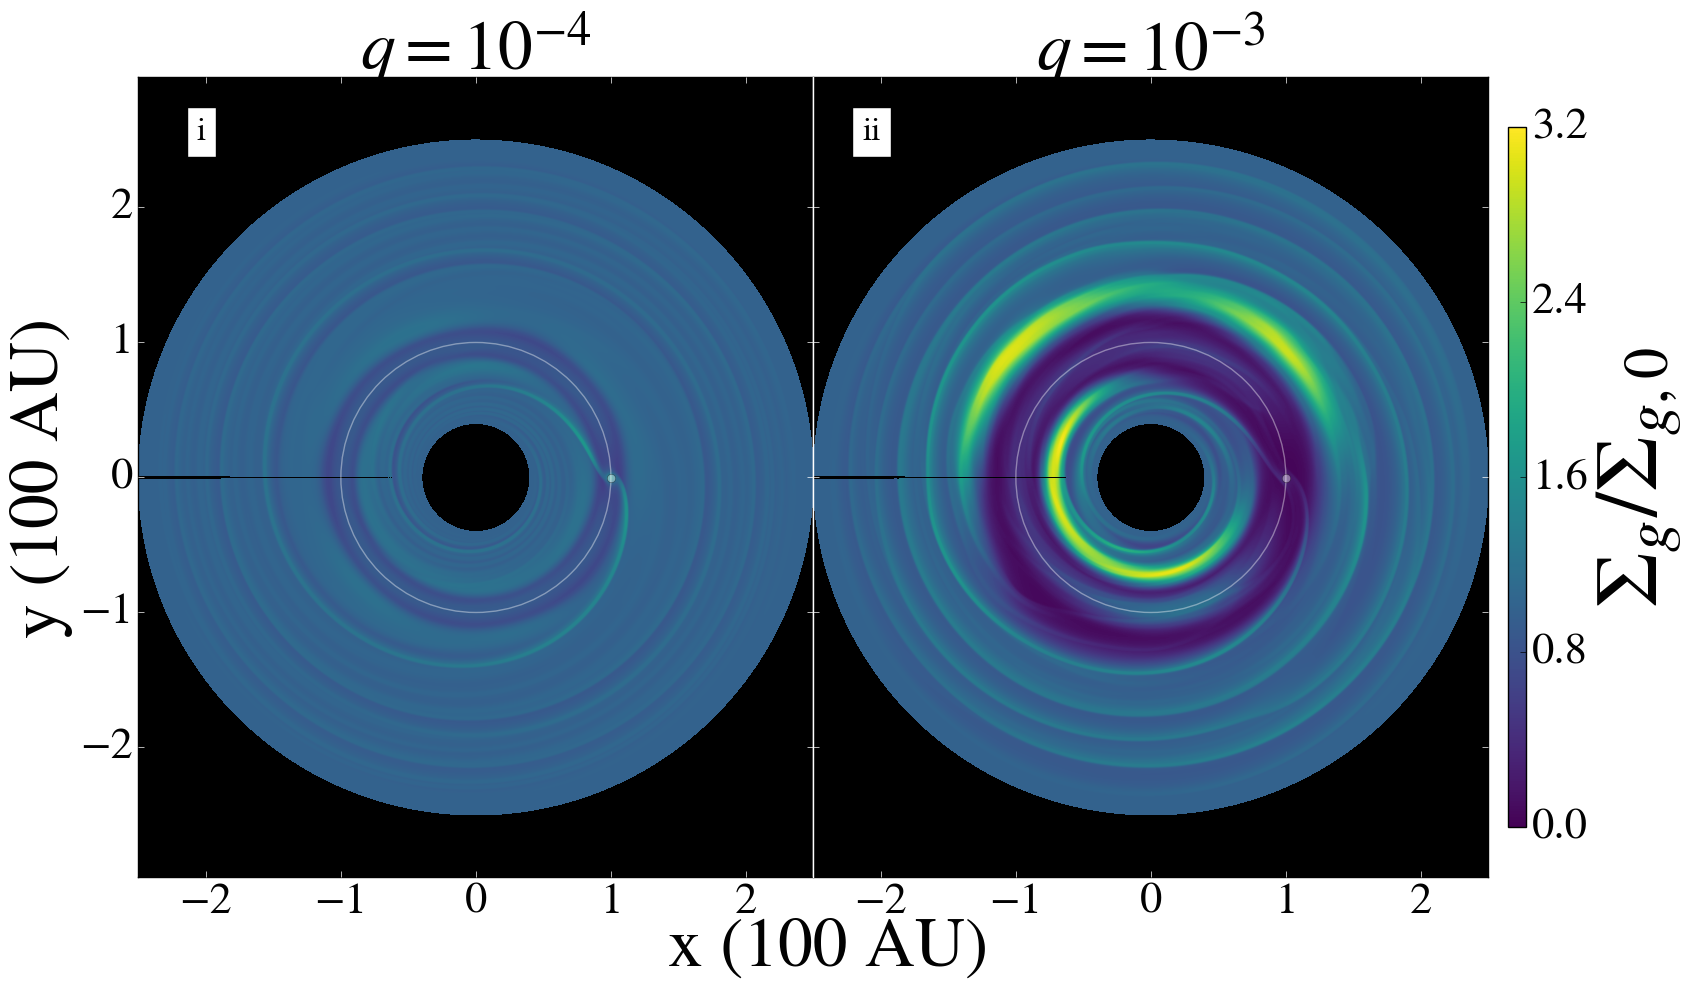
\includegraphics{dvbgasplotjupnep.png}}
    \resizebox{.7\textwidth}{!}{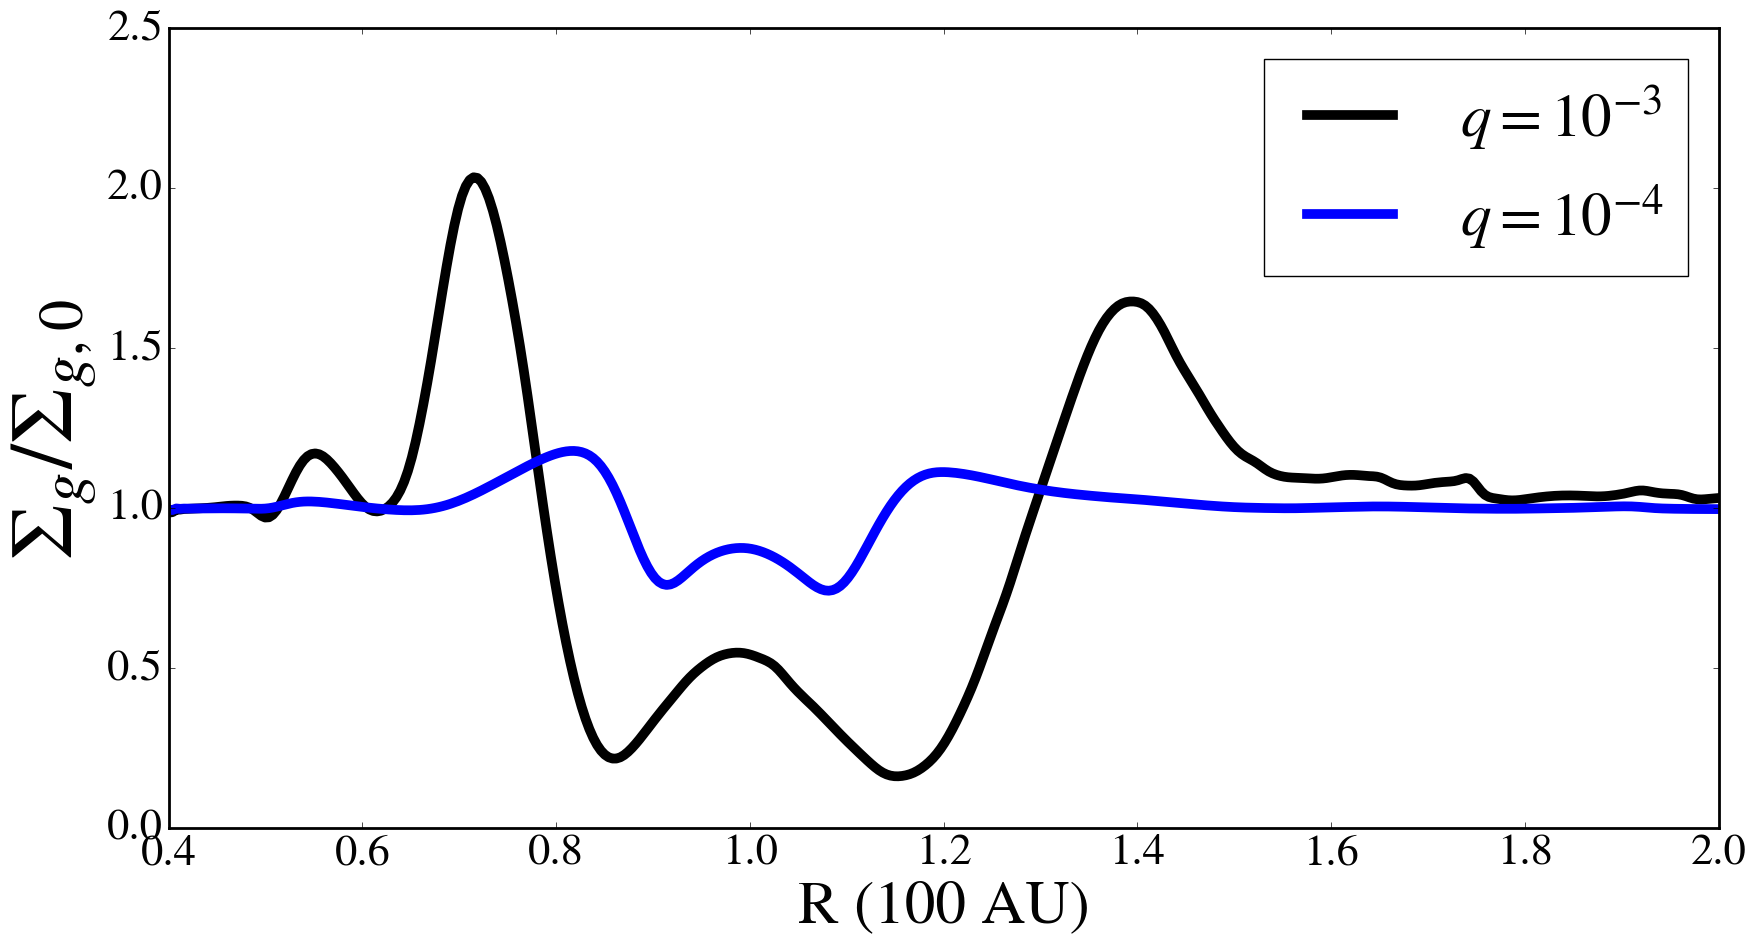
\includegraphics{dvbgasprofilesjupnep.png}}
    \caption{Fiducial run of a global disk containing only
      gas. \textit{Upper left:} Planet of mass ratio
      $q=10^{-4}$. \textit{Upper right:} Planet of mass ratio
      $q=10^{-3}$. Both planets carve a gap and generate a spiral in
      the gas. \textit{Bottom:} Averaged gas density as a function of
      radius from the star. The black curve represents a planet with
      mass ratio $q=10^{-3}$ and the blue curve represents
      $q=10^{-4}$. These models represent benchmarks against which we
      will compare models including dust and photoelectric instability.}
    \label{fig:devalborro}
  \end{center}
\end{figure} 


\section{The Effect of Dust}

In order to study the effects of the photoelectric instability in planet-disk interactions, we first need to investigate how the addition of dust will change the gap shape caused by a planet. The vast majority of works on planet-disk interactions asuume either a dust-free or gas-free scenario. Works that include both dust and gas, explore the regime of dust-to-gas ratios that are significantly below unity, where the dust is mostly passive, with the gas dominating the motion of the dust. This is perfectly fine for promordial disks, but to explore the mechanisms that happen in late-transition disks and debris disks with gas, we have to consider higher dust to gas ratios. We seek to find the point where dust backreaction generates a noticeable effect on the gap-carving process. We explore the parameters of dust-to-gas ratios $\epsi=\rho_d / \rho_g$ and planet-to-star mass ratios $q=M_p / M_\star$. Table one shows the majority of the simulations that we used and their letter or number indicator, which will be used in the figures for reference.  

\subsection{Dust Flattens the Gap Pressure Bump} \label{section:flattening}

In the upper panel of \fig{fig:gapjupiter}, we plot the gas density over the initial gas density as a function of distance from the star. The various curves correspond to different dust-to-gas ratios, ranging from 0 (dust-free) to 1, where the dust and gas are present in equal amounts. The scale height for all these plots is $h=0.05$. For the dustless case of 0 (black), up to $10^{-2}$, the gap does not deviate strongly. However, for $\varepsilon=10^{-1}$, and more strongly for $\varepsilon=1$, a significant deviation from the black curve is seen. This is the regime where dust begins to have a noticeable effect on the motion of the gas. In the lower panel, we plot the local dust-to-gas density. The dashed black line denotes the point where this quantity reaches unity. For $\varepsilon=0.1,1$ we note that the deviation in the gap in the upper panel coincides with the local dust-to-gas ratio reaches a value equal to, or close to 1. Therefore, we conclude that the gap carved in a disk deviates when the local dust-to-gas ratio reaches a value near unity.


\begin{figure}
  \begin{center}
    \resizebox{.9\textwidth}{!}{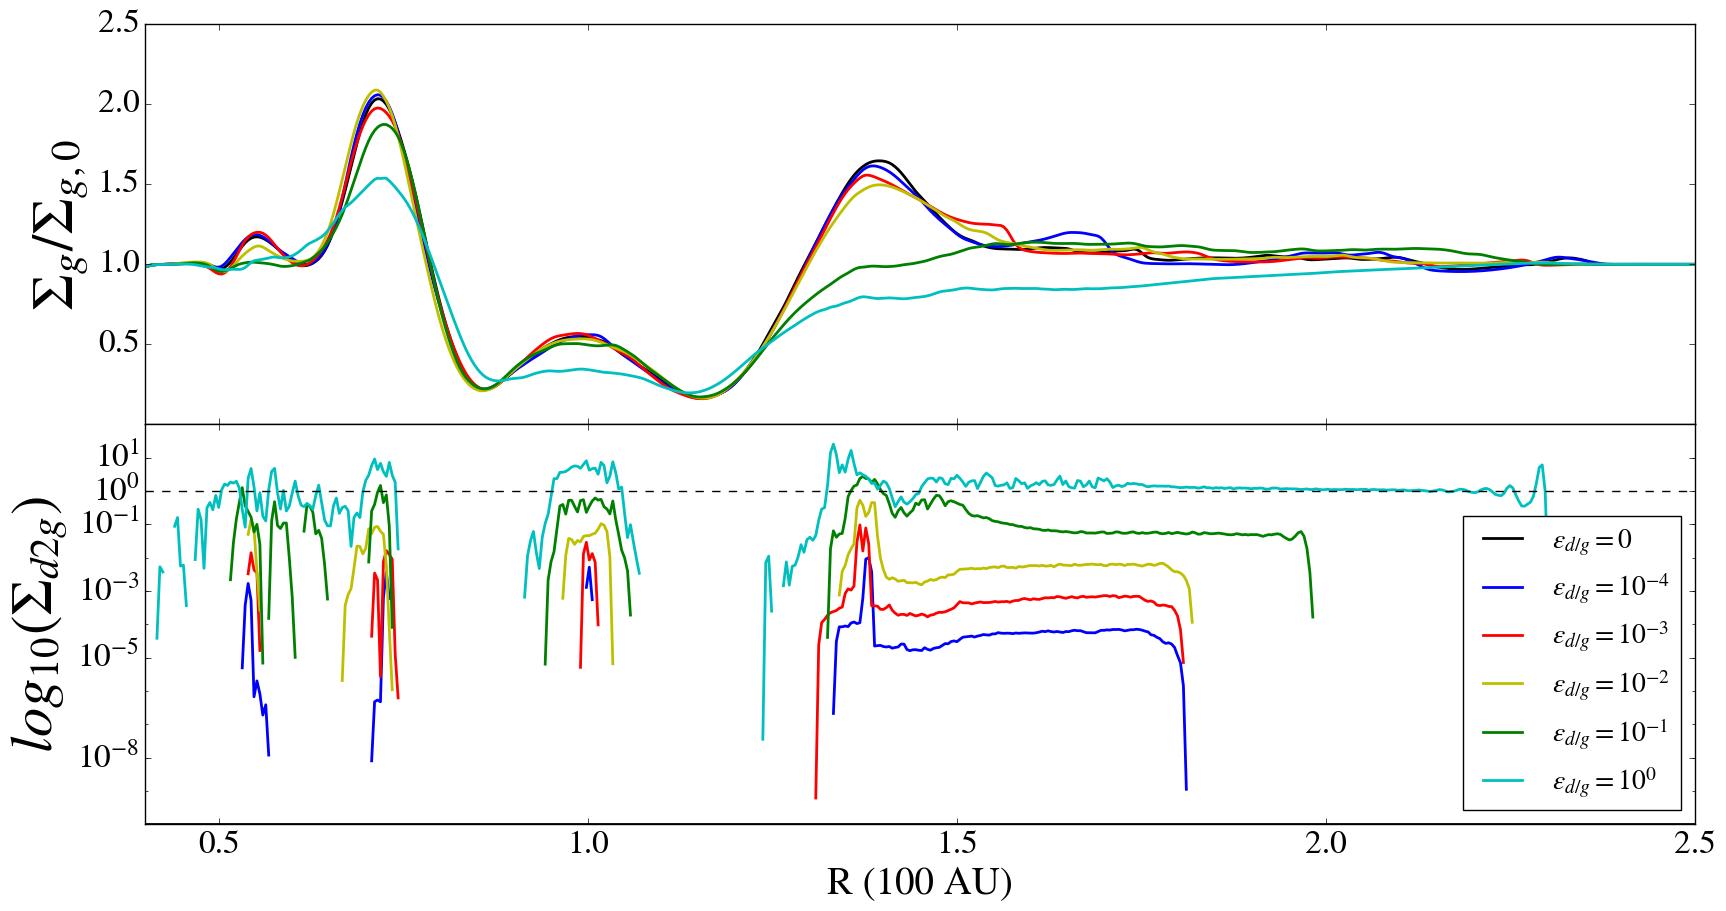
\includegraphics{qe-3gasd2g.png}}
    \caption{Effect of dust-to-gas ratio on the shape of planetary gaps. Snapshots are taken at 100 disk orbits for all cases. The top panel shows the gas gap shapes for different initial dust-to-gas ratios, for a Jupiter mass planet. The bottom panel shows the local dust-to-gas ratios. In the upper panel the black line shows a dustless model. As dust-to-gas ratio increases, the pressure bump in the inner gap-edge becomes suppressed, and the bump in the outer gap-edge is nearly washed out. Inspecting the lower plots, the deviation from the dustless case happens when the local dust-to-gas ratio approaches unity. This is expected, as the backreaction of the dragforce comes to heavily influence the gas motion. This threshold is easily reached in the pressure bumps of the planetary gap edges for the runs with initially high dust-to-gas ratios. Given enough time, disks with $\varepsilon=10^{-2}$ (and lower) will reach unity, if the disk is large enough and the pebbles drift continously. The particle drift is enhanced by the planeraty gap and a global negative pressure gradient.}
  \label{fig:gapjupiter}
  \end{center}
\end{figure}


\begin{figure}
  \begin{center}
    \resizebox{.9\textwidth}{!}{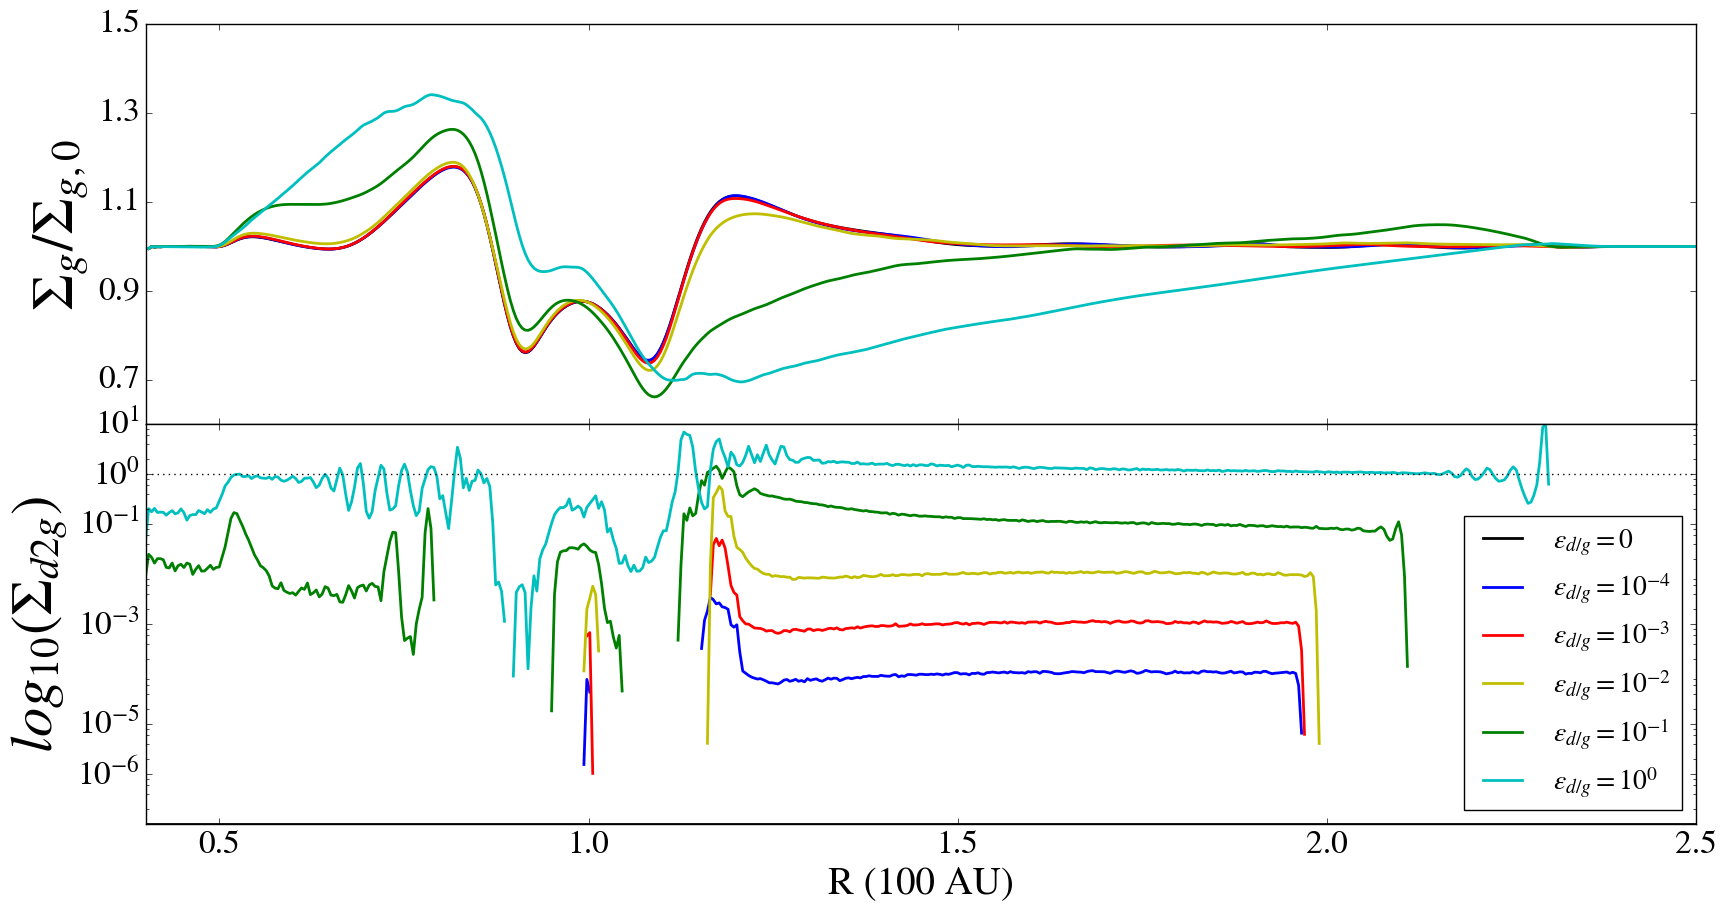
\includegraphics{gap_shapes_neptune_mass.png}}
  \end{center}
  \caption{Same as \ref{fig:gapjupiter} but for $q=10^{-4}$. A high dust-to-gas ratio again causes the shape of the gap to deviate from the dustless case. The two highest dust to gas ratios are affected as well as the $\varepsilon=0.001$ case. The effect of the inner bump anticorrelate with the Jupiter case, this is explained in \textbf{INSERT SECTION HERE}.}
  \label{fig:gapneptune}
\end{figure}


\subsection{Dependency on Extent of Mass Reservoir}

Due to the effect of the global negative pressure gradient, dust grains in the outer disk move drift inwards. As time progresses, the drift is enhanced due to the pressure that is generated by the planetary gap. Notice the strong dependency of the drift speed on the dust-to-gas ratio. Particles that start with a high dust-to-gas ratio drift inwards the slowest because they are strognly affecting the gas.\par

We could conclude, that if the drift continues, and all grain pile up at the gap edge, any initial dust-to-gas ratio will eventually accheve a dust-to-gas ratio of unity. Even for a simulation that begun with $\varepsilon=10^{-2}$ (yellow line), it is close to reaching a value that is close to one. If they can reach this value based on the dust drift alone, then the constraint put on the disk is correlated to the mass reservoir in the disk. 

\subsection{Differences in Inner Disk for Different Planet Masses \& Dust-to-Gas Ratio}

Another feature seen \fig{fig:gapneptune} \& \fig{fig:gapjupiter} is the reversal at the inner bump for higher dust-to-gas ratio for the two planetary masses. In the outer disk, both planets suppress the gap edge as the dust-to-gas ratio increases. However, in the inner disk, the Neptune-mass planet increases the gap height with increase in dust-to-gas ratio. This behavior is not present fot the Jupiter-mass planet.\par

\begin{figure}
  \begin{center}
    \resizebox{.8\columnwidth}{!}{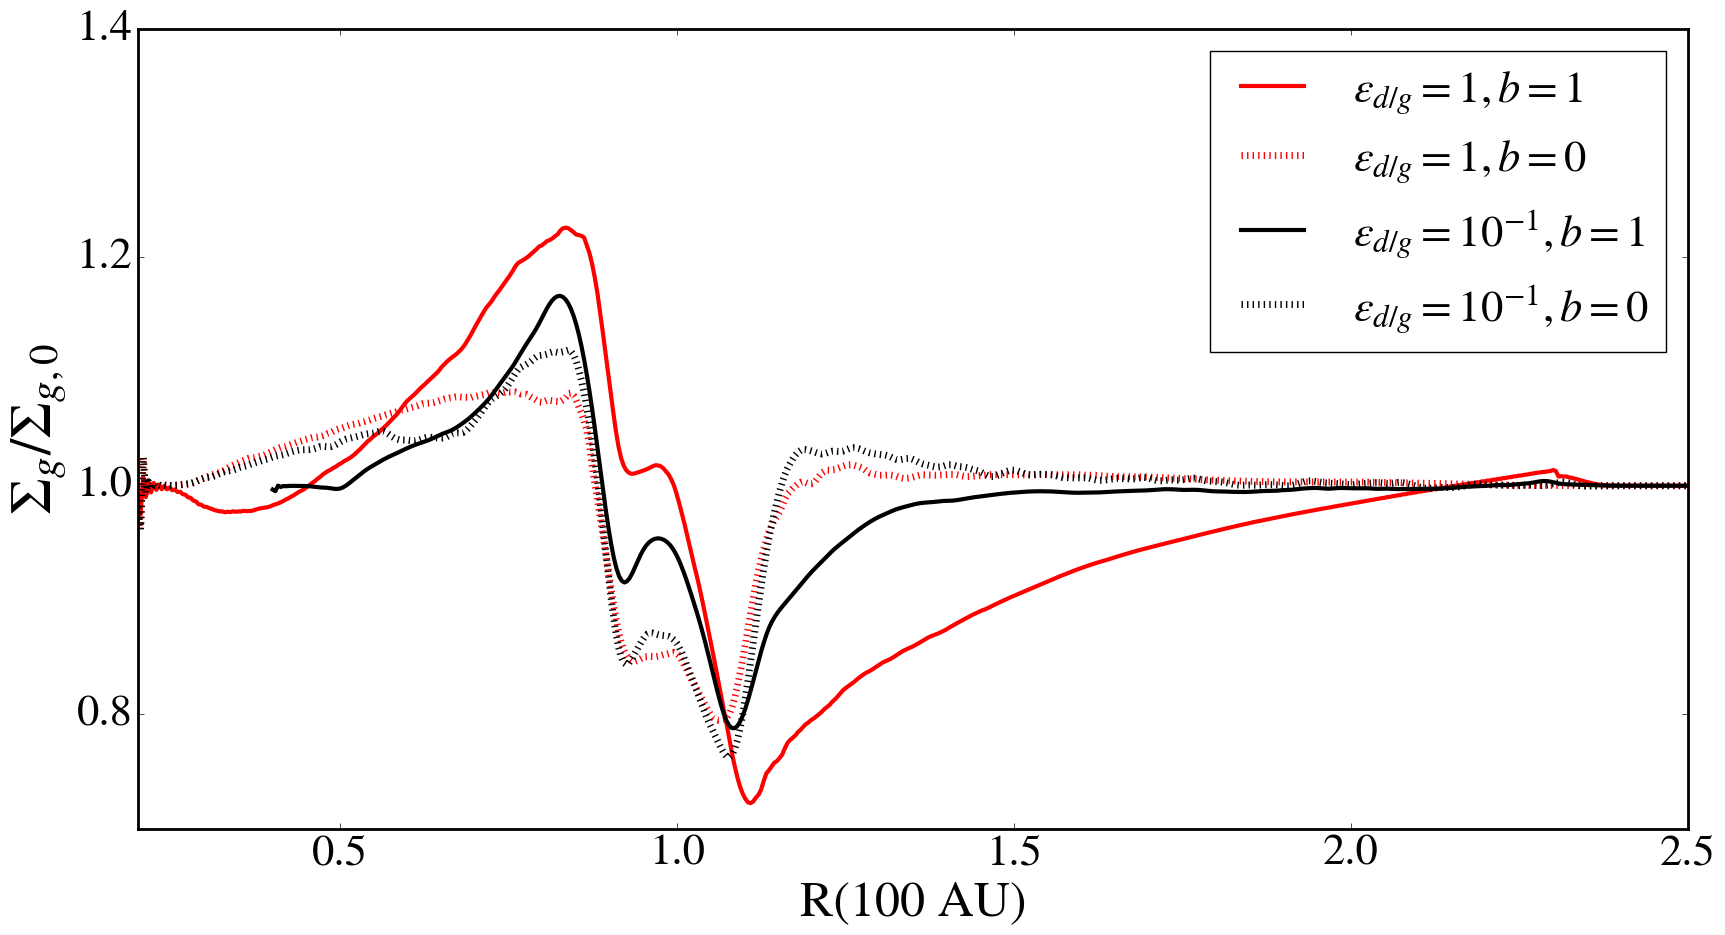
\includegraphics{figures/nep_rhoprof_nopgrad.png}}
  \end{center}
  \caption{The effect of the particle drift and angular
    momentum conservation in the gap profile of a
    Neptune-mass planet. The red lines show runs with
    $\varepsilon=1$. The black lines show runs with $\varepsilon=0.1$. Solid lines have $b=1	$ ($b$ is
    the power law of the temperature, giving a global negative pressure
    gradient); the dashed lines are control runs that correspond to $b=0$, with no global
    negative pressure. The control runs are similar, with the
    higher-dust to gas ratio showing a small depression. However, when
    drift is included, to conserve angular momentum the gas is pushed
    outwards. For higher dust-to-gas ratios (solid red line),
    more gas is pushed outwards than for lower dust-to-gas ratio (black
    solid line).}
  \label{fig:drift}
\end{figure}

The difference in this behavior is due to the particles drifting inwards within the disk. This effect is seen in \Fig{fig:drift}. The red lines show runs with a dust-to-gas ratio of 1, and the black lines show runs with dust-to-gas ratio of 0.1. Solid lines have a $b$ value of 1. The parameter $b$ is the power law of the temperature, which gives a global negative pressure gradient. The dashed lines correspond to a $b$ value of 0, where there is no negative global pressure. If we exclude the drift, the simulations are similar, where a dust-to-gas ratio of 1 causes a smaller pressure bump than 0.1, due to the flattening mentioned in Section~\ref{section:flattening}. Runs with a global pressure show significant differences. As particles drift inward, in order to conserve angular momentum, they push the gas outwards. For higher dust-to-gas ratios more gas is pushed outwards than for lower ratios. This effect is seen for the Neptune-mass planet, but not the Jupiter-mass planet. This is because the Jupiter-mass planet carves out a much larger gap from an ealier time, resulting in a less amount of gas being present to be pushed outward. 

\begin{figure}
  \begin{center}
    \resizebox{.9\textwidth}{!}{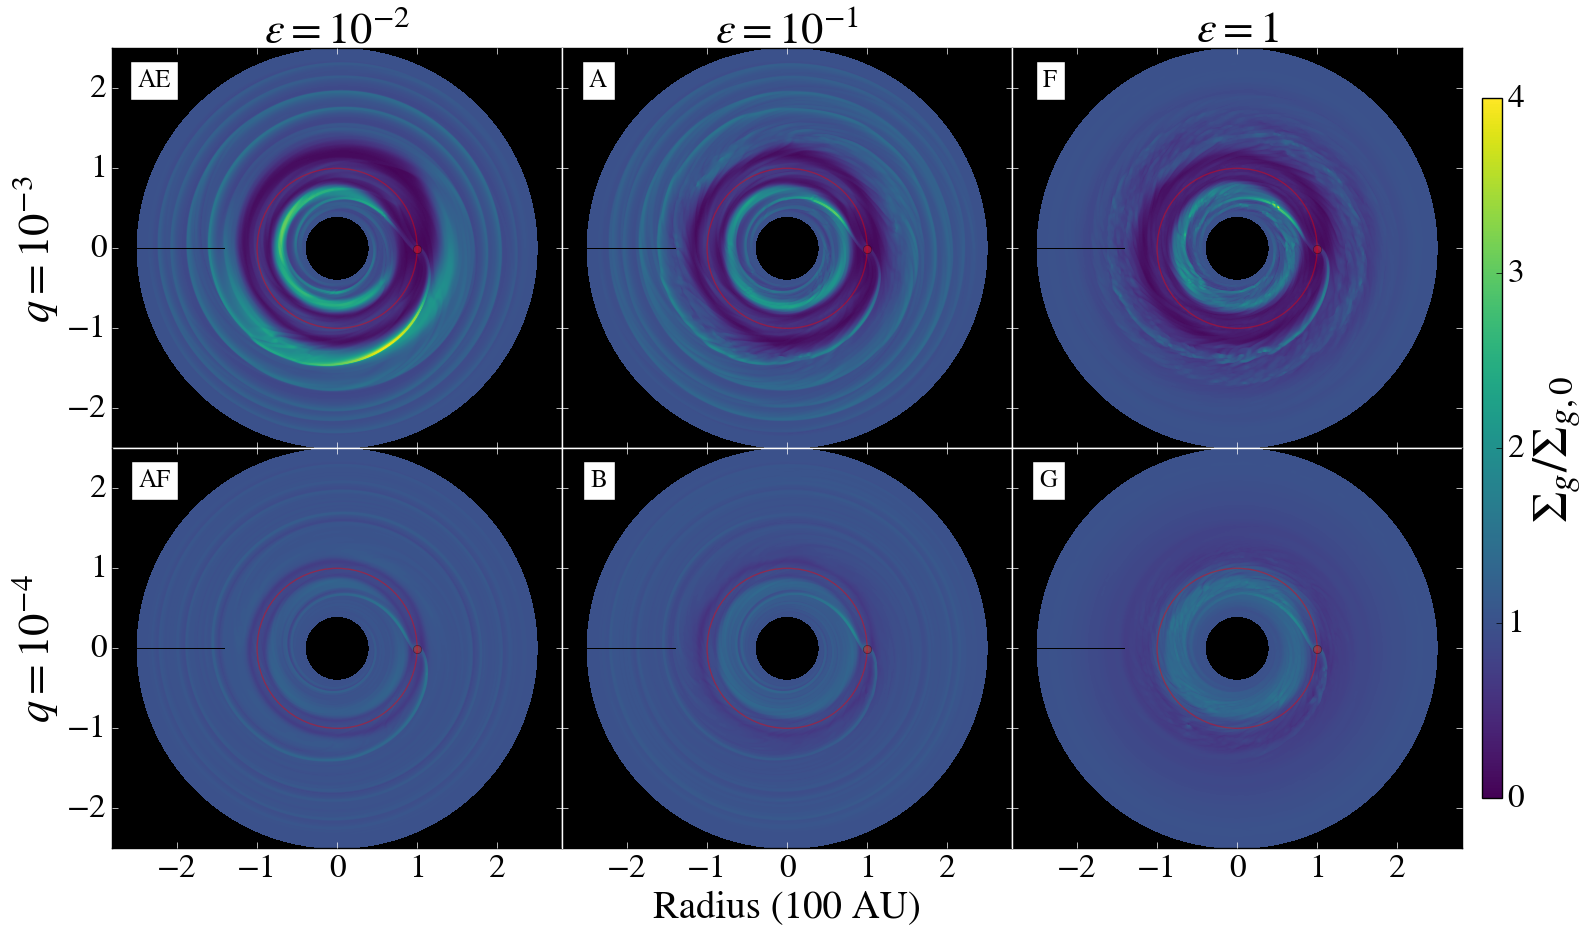
\includegraphics{global_gas_changes_in_epsilon_both.png}}
  \end{center}
  \caption{Two dimensional visualization of the effect of dust-to-gas ratio in \Fig{fig:gapneptune} \& \Fig{fig:gapjupiter}. The plots show the gas density for a disk with 	    planet mass ratio $q=10^{-3}$ (Top) and $q=10^{-4}$ (Bottom), with dust-to gas ratios ($\epsi=10{-2}, 10^{-1}, 1$) increasing towards the right. For $\epsi=10^{-2}$, the dust concentration remains low and the gas is unaffected, with the spiral and gap edges remaining mostly smooth as in the dustless case in \Fig{fig:devalborro}. However, for $\epsi=0.1$, the effect is visible at the gap edges and the spiral as they become less laminar and more turbulent-like. In the $\epsi=1$ case, the spiral breaks up into eddies, similar to the behavior of cigarette smoke.}
  \label{fig:jupnepd2g}
\end{figure}


In \Fig{fig:jupnepd2g} we show 2D plots of the gas density for planet masses $q=10^{-3}$ (upper) and $q=10^{-4}$ (lower). Dust-to-gas ratios $\varepsilon=10^{-2}, 10^{-1}, 1$ are shown from left to right columns. The effect of a low dust-to-gas ratio is barely noticeable for the case of $\varepsilon=10^{-2}$ \& $q=10^{-4}$, when compared to \ref{fig:devalborro}. For dust-to-gas ratio of 0.1, the gas in the gas in the disk becomes more turbulent-like in at the gap edges. The spirals that are caused in the dustless case are smooth and laminar, but as they reach this threshold they become visibly turbulent. Increasing the dust-to-gas ratio to unity, the wake and gaps look even more turbulent, in a pattern resembling cigarette smoke.

Considering only debris disks and $\mu m$ grains, this particular result depends only on the Stokes number and dust-to-gas ratio. It could therefore be applicable to primordial protoplanetary disks if pebbles and boulders ever reach these high values of $\epsi$.

\section{Disk with $\epsi=10^{-1}$ and $h=0.05$}

\begin{figure}
  \begin{center}
    \resizebox{.8\textwidth}{!}{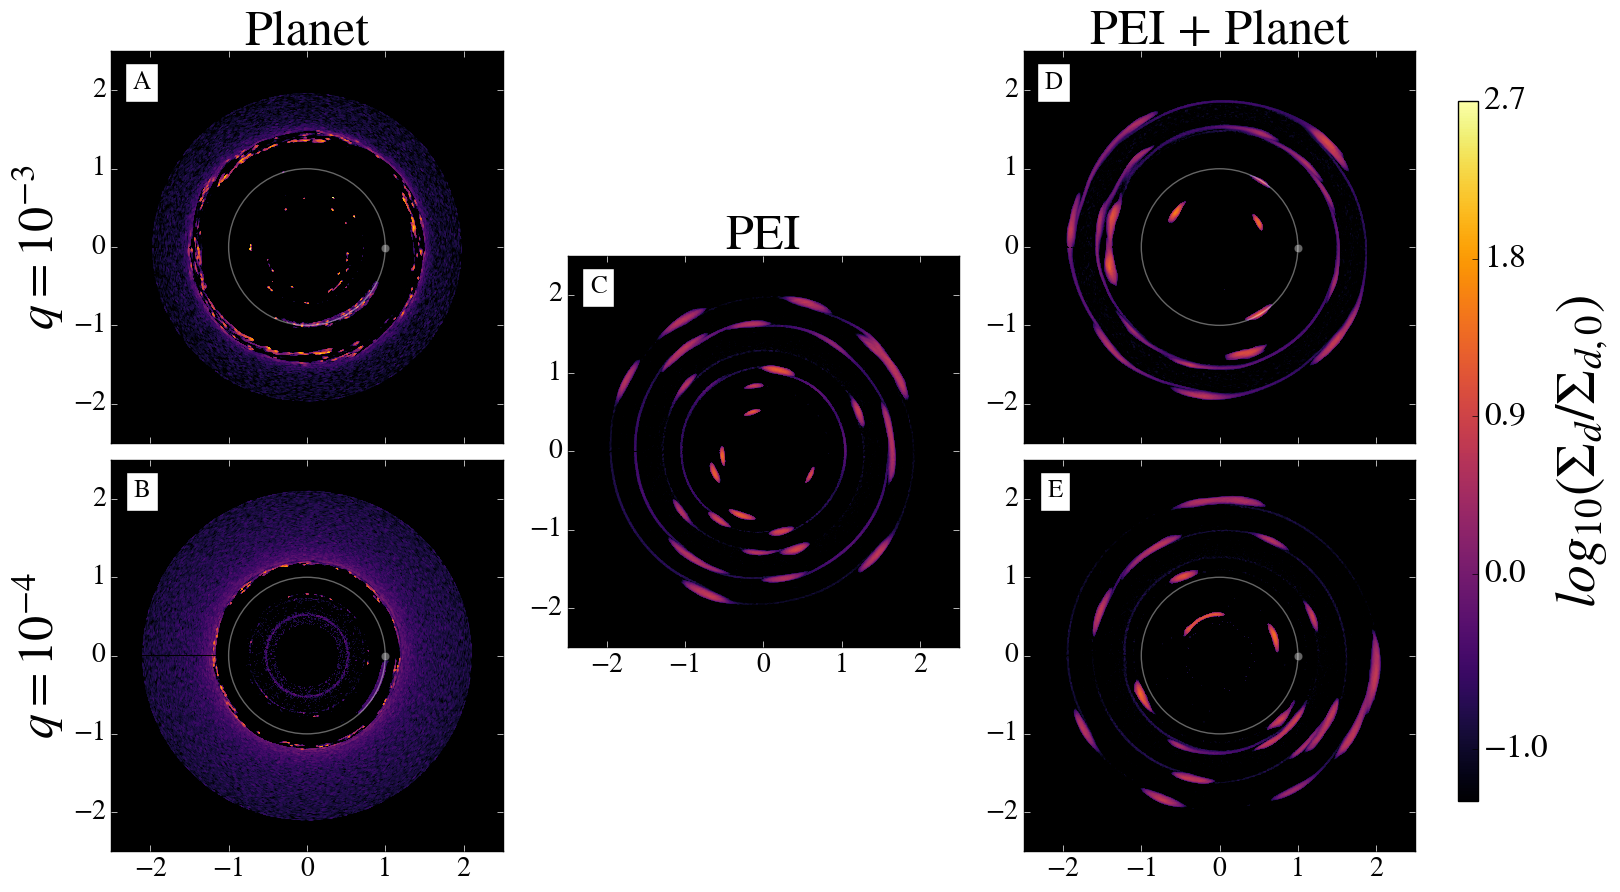
\includegraphics{./05_10-1_dust_global.png}}
    \resizebox{.8\textwidth}{!}{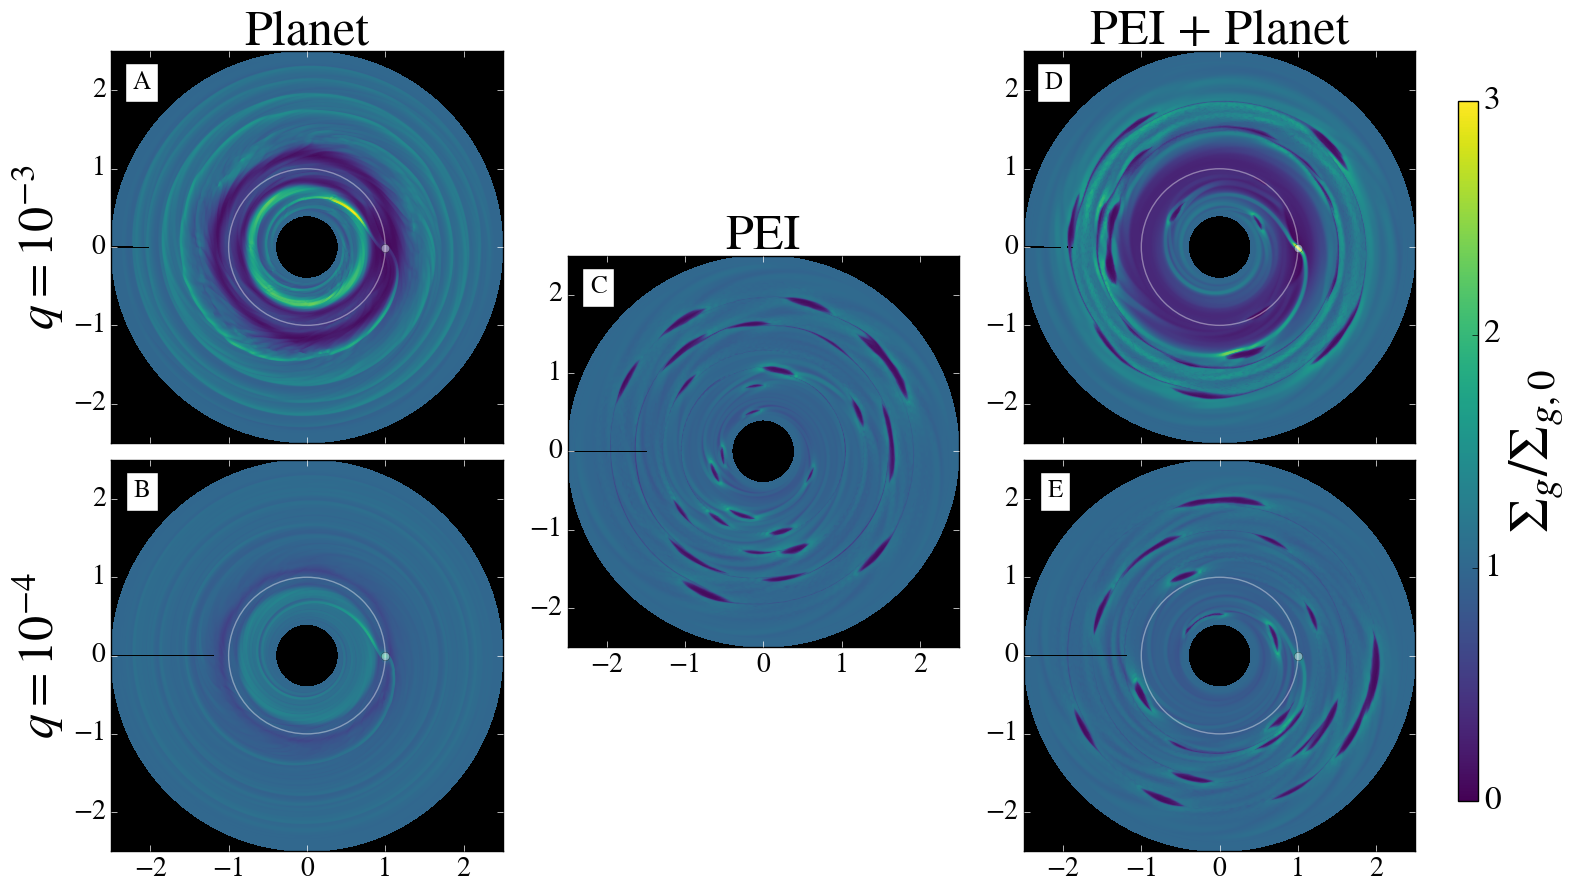
\includegraphics{./05_10-1_gas_global.png}}
  \end{center}
  \caption{Dust (upper panels) and gas (lower panels) in
    a disk with initial dust-to-gas ratio $\varepsilon=10^{-1}$. The top row shows results for a disk with a planet of mass ratio $q=10^{-3}$ and the bottom row shows results for mass ratio $q=10^{-4}$. The first column shows the effect of planet with no photoelectric heating. The middle column, labeled ``PEI'', shows the effect of the photoelectric instability on its own. The last column shows the combined effect of photoelectric instability and a planet. The most striking feature of this comparison is that the $q=10^{-4}$ planet with PEI is virtually indistinguishable from the PEI alone (the middle case). The main feature that makes the $q=10^{-3}$ distinguishable in the midst of PEI structures is the deep and clear planetary gap. We conclude that when photoelectric heating is included, we find that the photoelectric instability obscures structures induced by planets unless the planet's mass is sufficiently large to carve a noticeable gap. The plots are shown after 100 planetary orbits.}
  \label{fig:eps01dustgas}
\end{figure}

In \Fig{fig:eps01dustgas} we plot the dust on the top and the gas on the bottom for a disk with $h=0.05$ and an initial dust-to-gas ratio of $\epsi=0.1$. For each panel, the left column are simulations containing an embedded planet and no photoelectric heating, the middle columns are simulations of a disk containing photoelectric heating but no embedded planet, and the right columns are simulations for disks containing both and embedded planet and photoelectric heating. The top and bottom rows correspond to a Jupiter-mass and Neptune-mass planet, respectively.

The top panels show the local dust density divided by the initial dust density on a logarithmic scale. The cavitites carved in Run A \& B manifest differently, with run A having noticeably larger gap whe compared to run B. Run A also has an overall lower dust density throughout the disk when compared to run B. These well known results (\textbf{Paardekopper \& Mellema 2004} are expected as a higher-mass planet clears its orbit.)

Run C demonstrates the effects of photoelectric heating on a disk. The structures created are similar to those of (\textbf{Lyra \& Kuchner 2013}), showing rings and incomplete arcs.

Runs D and E correspond to a disk subject to photoelectric heating and containing a planet. Run E, which shows the Neptune analog, is nearly identical when comparing to the control run in C, containing the same structures that are shown in the instability case. We can conclude that the addition of a Neptune-mass planet does not noticeably alter the shape or number of structures from the pure instability case. Run D, which contains a Jupiter-mass perturber, shows larger arcs and a discernable cavity. This is another novel result. When photoelectric heating is included, the photoelectric heating obscures structures induced by planets, unless the planet's mass is sufficiently large enough to carve a noticeable gap. The shape of the structures for this case are also changed when compared to the Neptune case. This is likely due to the stronger eccentricity stirring at mean-motion resonances with higher plaetn mass (\textbf{Murray \& Dermott 1999; Zhu et al. 2014}).

The bottom plots show the same plots as above, but for the gas, where the local gas density is divided by the initial gas density on a linear scale. The most pronounced feature that we see is the anticorrelation of dust and gas, where a large concentration of dust will lead to gas depletion. Reiterating for the gas case, we see that a Jupiter-mass perturber carves a larger gap and leads to a more prominent spiral. The spiral launced from the Nptune-mass planet is almost lost in the midst of structures being generated by the photoelectric instability.

\begin{figure}
  \begin{center}
    \resizebox{.45\textwidth}{!}{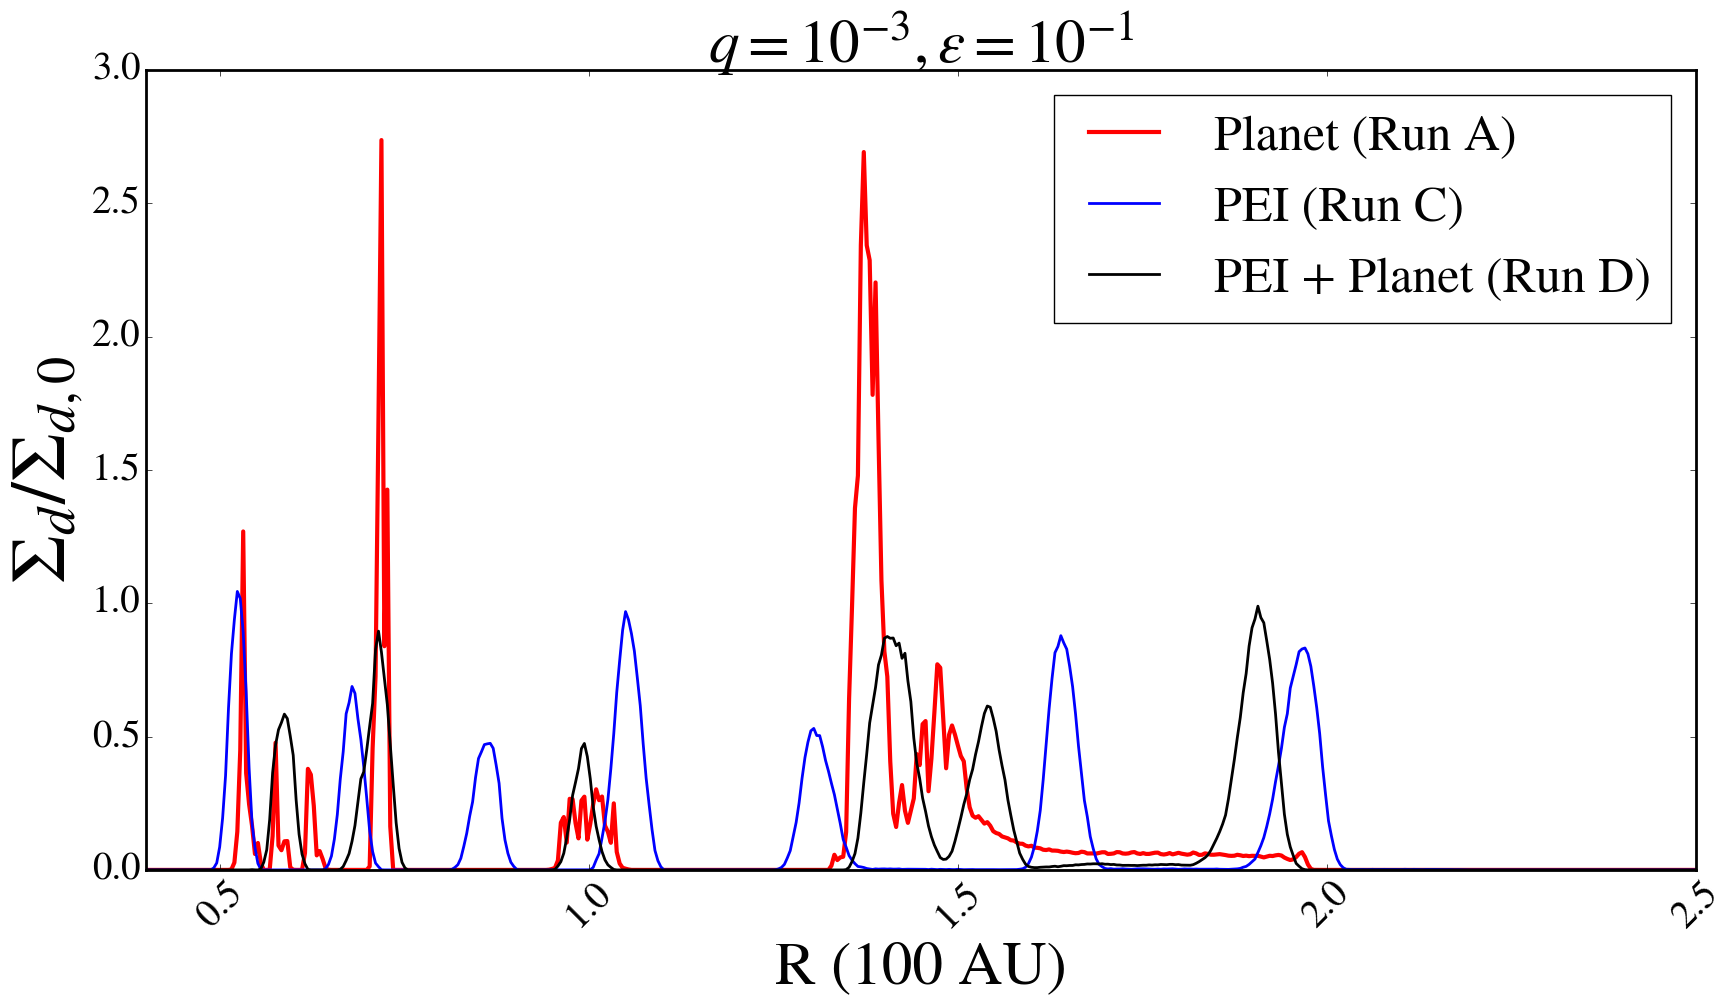
\includegraphics{./05_m3_10-1_dust_profile.png}}
    \resizebox{.45\textwidth}{!}{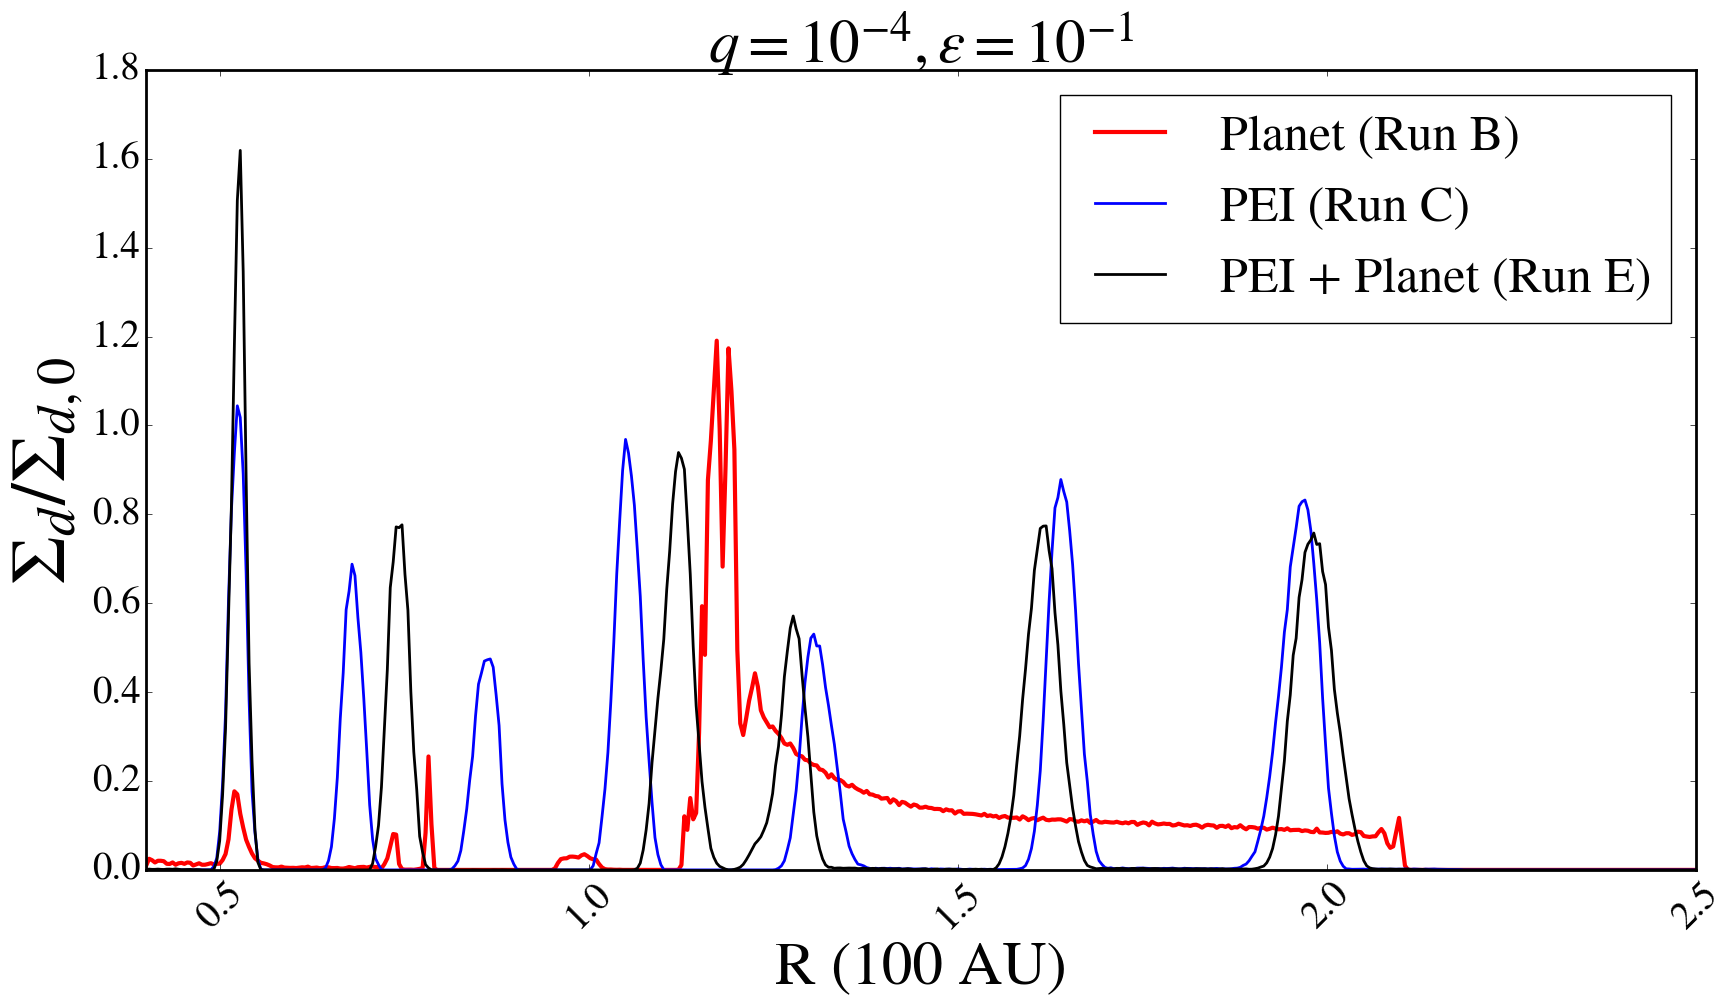
\includegraphics{./05_m4_10-1_dust_profile.png}}
  \end{center}
  \caption{Azimuthal average of the dust density for the simulations shown in
    \ref{fig:eps01dustgas}. The left plot shows the $q=10^{-3}$ case, the
    right plot shows the $q=10^{-4}$ case. The cases of planet only
    (red line) and planet + instability (black line) both have a large gap in the dust, centered at $r=1$, where the
    planet is located. The pure PEI case (blue line) shows structure inside the
    predicted location of the gap. The lower mass planet also carves a
    dust gap, but the pure instability and combined case coincide
    almost exactly. The planet cannot easily be disentangled
    from the instability in this case.}
  \label{fig:eps01dustprofile}
\end{figure}   


In \Fig{fig:eps01dustprofile}, we plot an averaged linear dust density as a function of radius from the star. The left panel coincides with a Jupiter-mass and the right with a Neptune-mass planet. On the left panel, the combined case in solid black, creates larger concentration of dust than the pure instability case, shown in the solid blue. Additionally, we see that the more massive planet (left), carves a larger gap at the location of the plaenet (100 AU). The width of the gap carved is on the order of 50 AU. For the Neptune case, the blue and black lines coincide in various locations throughout the disk. At the location of the planet (100 AU), there is no discernable gap. This echoes our conclusion that a planet must carve a substantial gap in the dust, allowing planet-induced structures to be disentangled from those of the photoelectric instabilty. The shapes shown here can be used in tandem with actual observations to narrow down the possibility of an embedded planet in a disk where the gas is subject to photoelectric heating.

\section{Disk with $\epsi=1$ and $h=0.05$}

\begin{figure}
  \begin{center}
    \resizebox{.8\textwidth}{!}{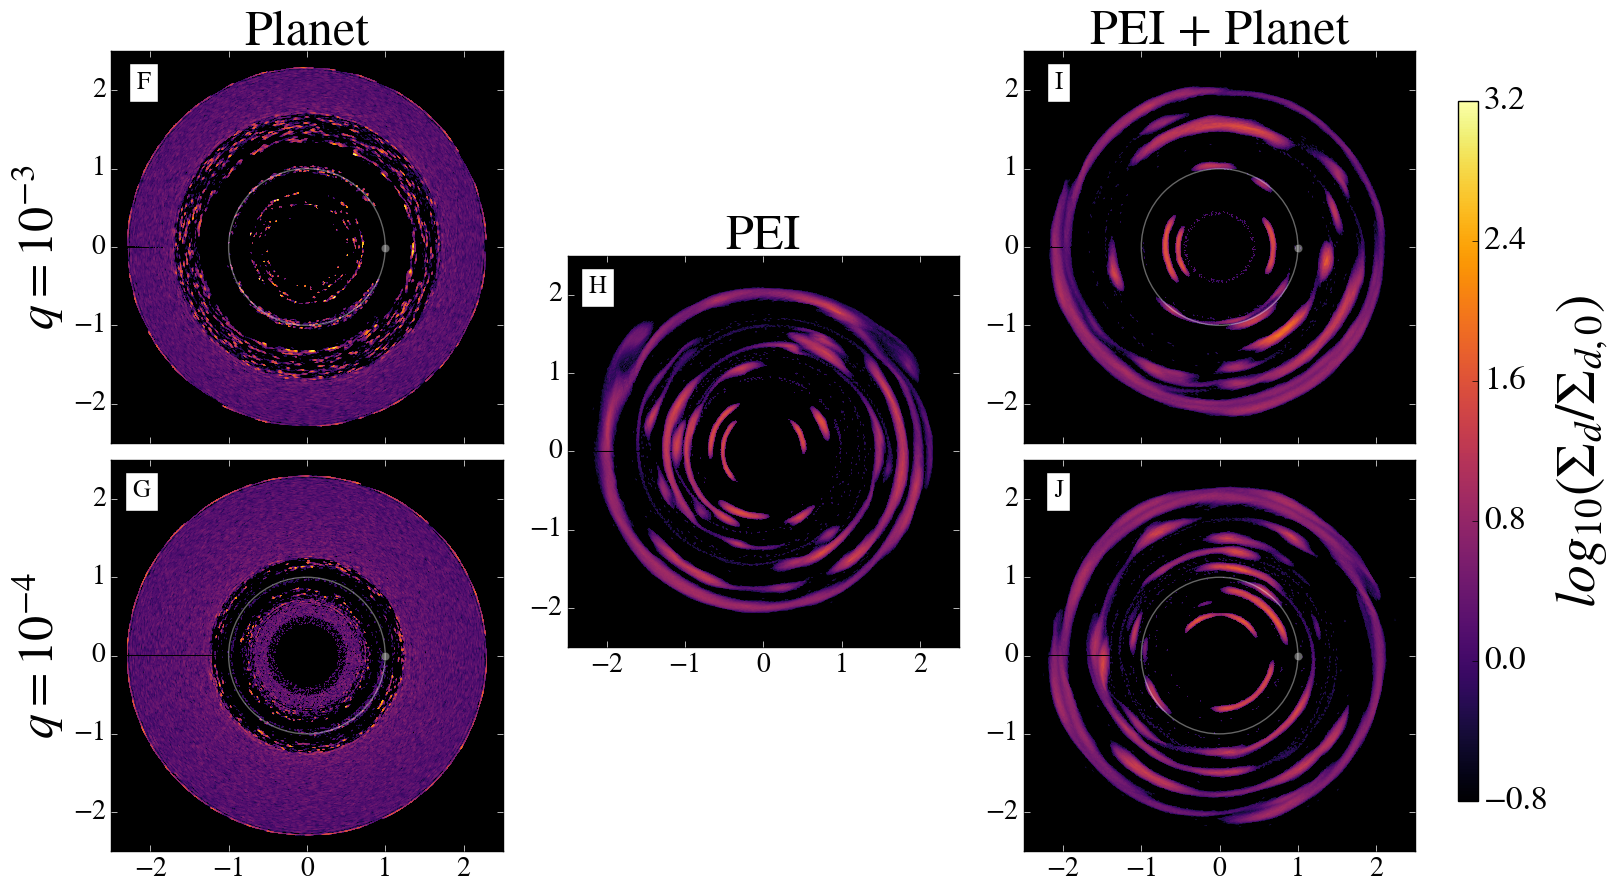
\includegraphics{./05_10-0_dust_global.png}}
    \resizebox{.8\textwidth}{!}{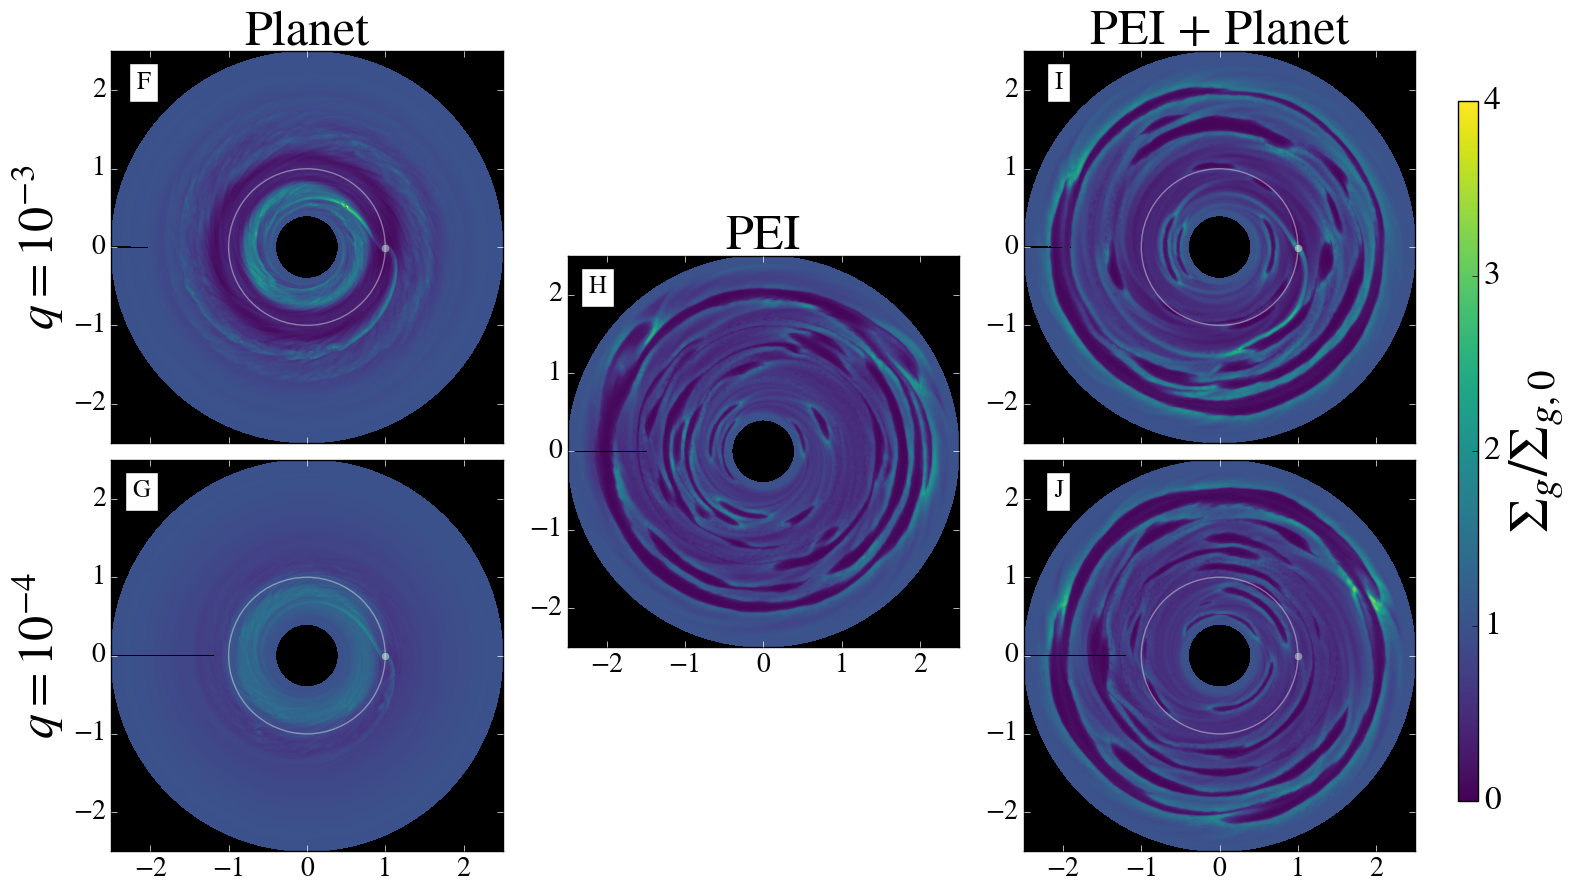
\includegraphics{./05_10-0_gas_global.png}}
  \end{center}
  \caption{Dust (upper panels) and gas (lower panels) for a disk with
    dust-to-gas ratio of unity. The disk aspect ratio is
    $h=0.05$. With the increased dust-to-gas ratio (and stronger
    effect of the drag force backreaction), the planet-only case shows increased
    turbulent-like behavior, and the wake has the appearance of
    cigarette smoke. The middle panels shows a simulation with PEI
    only. With more dust, the structures are different than in
    \Fig{fig:eps01dustgas}, which is to be expected, given
    more photoelectric heating and more backreaction.
    In the combined case (right panels), the plots suggest that
    the simulation with the higher mass planet is more depleted in
    grains than the simulation with the lower mass planet. We quantify
    this result in \Fig{fig:eps1dustprofile}. In the gas
    plots (lower panels) the spiral wake of the higher mass planet is
    visible.}
  \label{fig:eps1dustgas}
  \end{figure}

\begin{figure}
  \begin{center}
    \resizebox{.45\textwidth}{!}{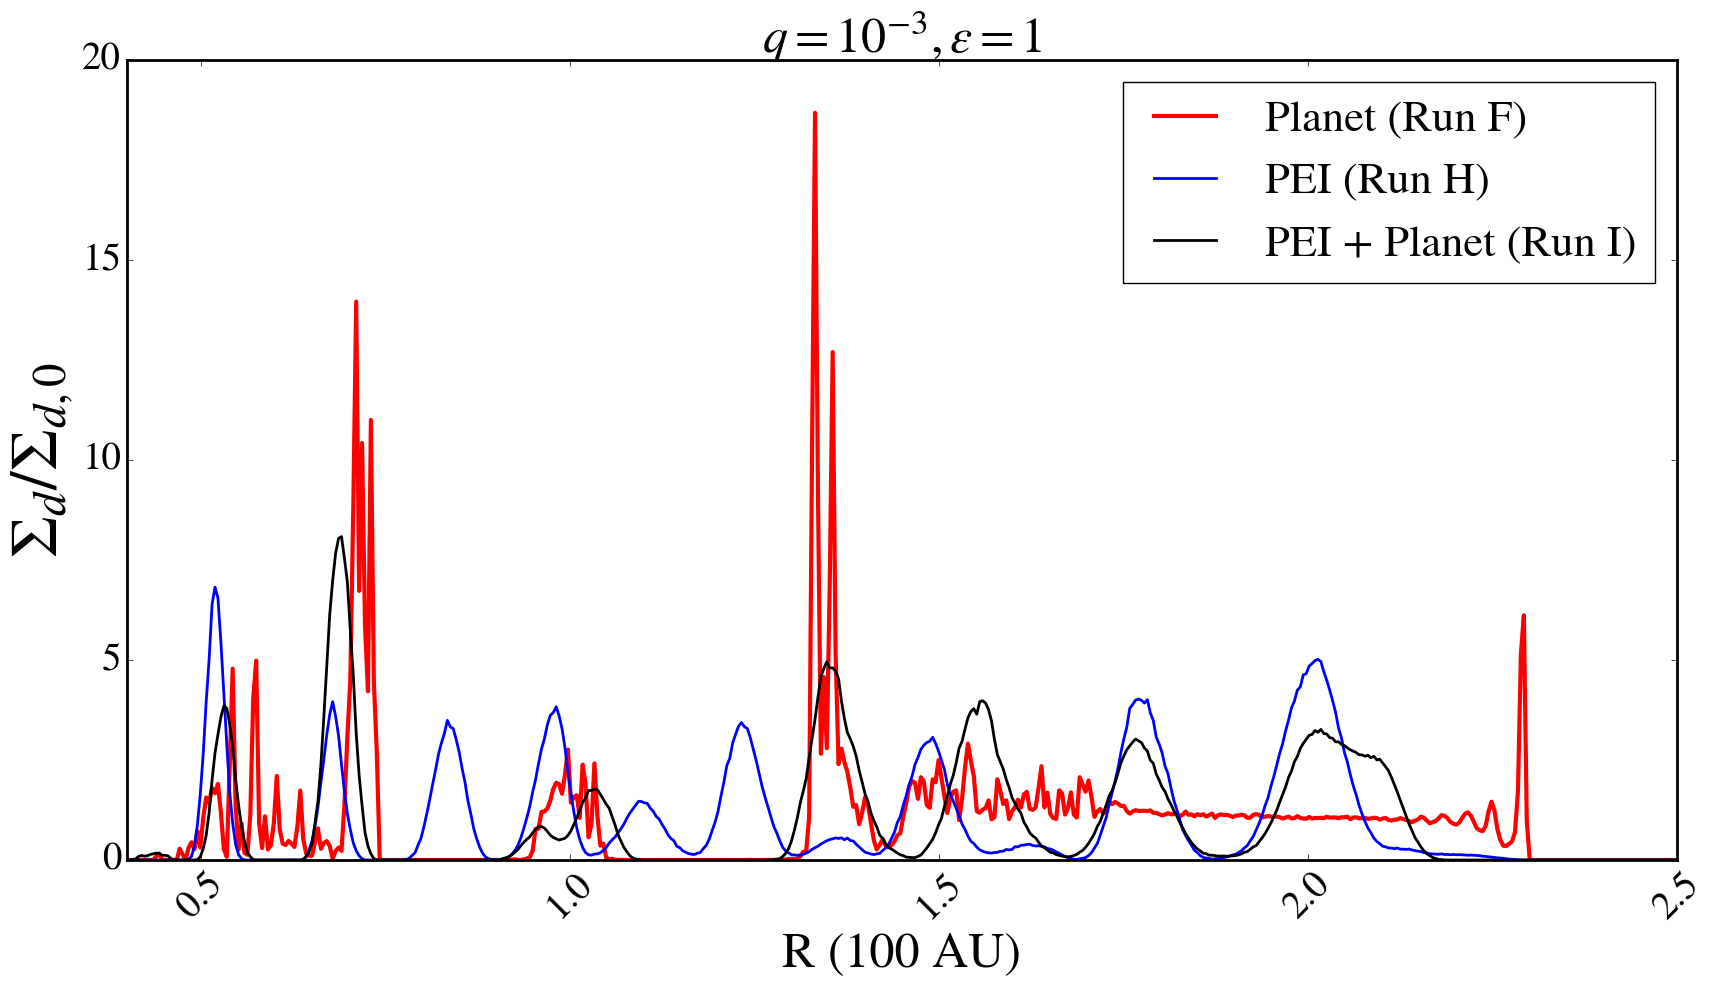
\includegraphics{./05_m3_10-0_dust_profile.png}}
    \resizebox{.45\textwidth}{!}{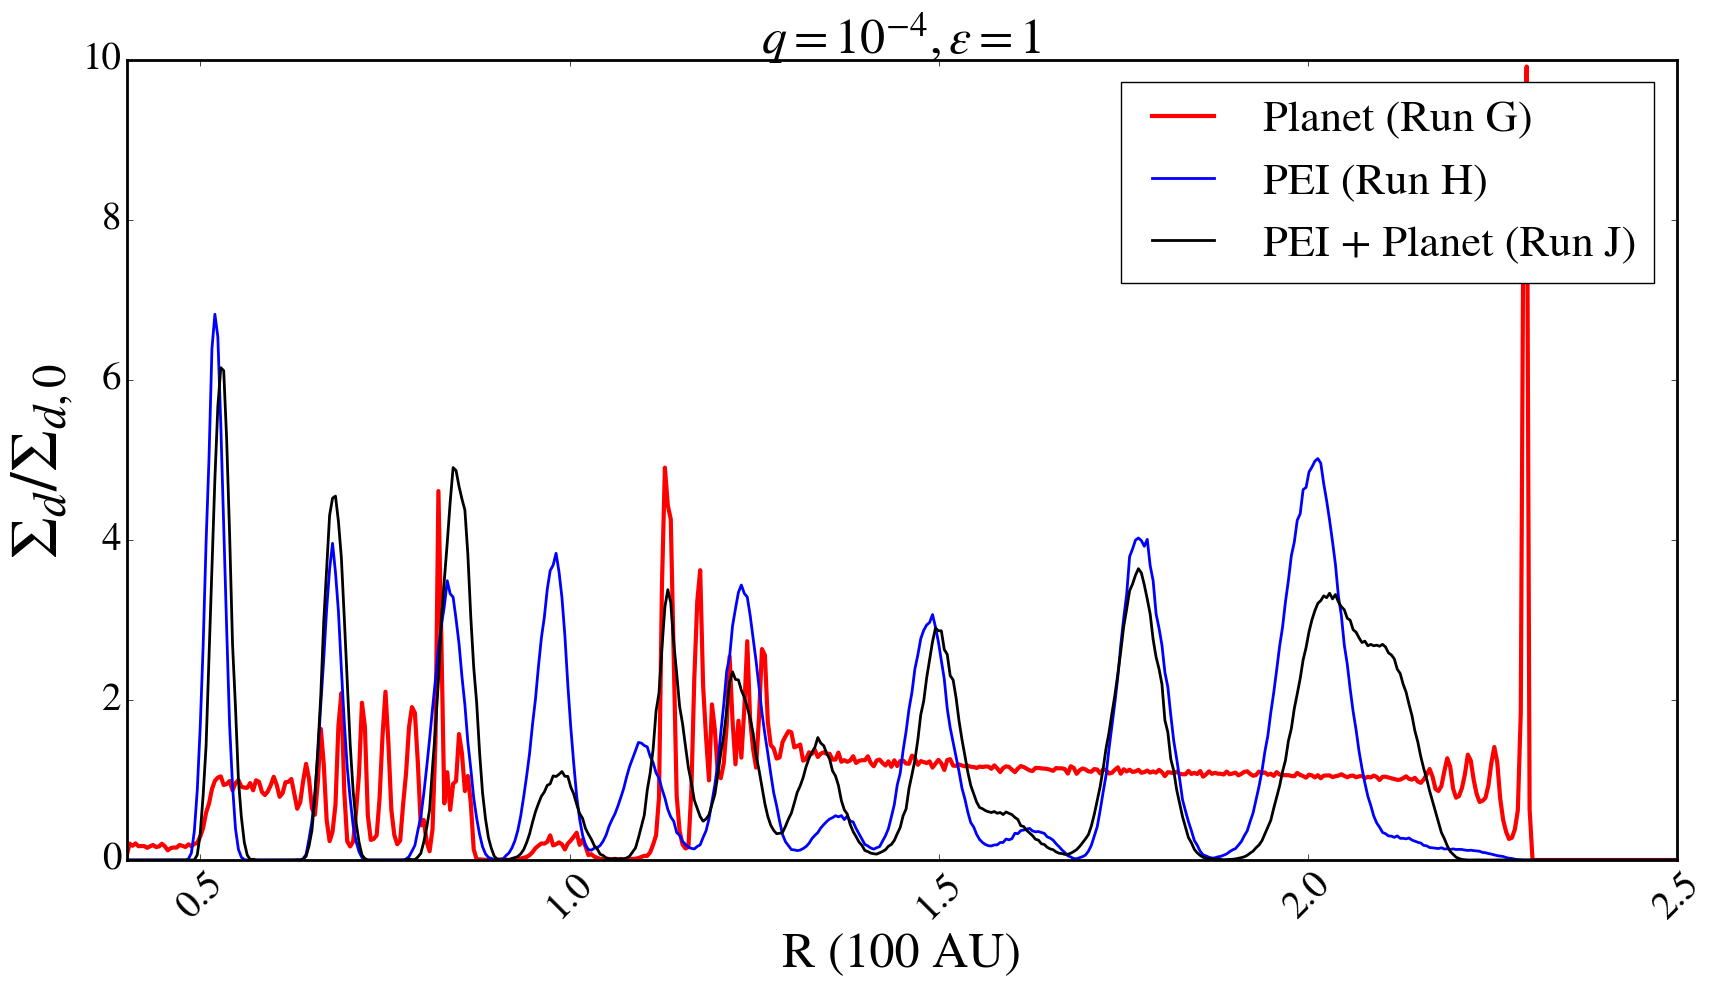
\includegraphics{./05_m4_10-0_dust_profile.png}}
  \end{center}
  \caption{Same as \Fig{fig:eps01dustprofile} but for $\varepsilon=1$. The
    simulations with the Jupiter-mass planet case shows a
    discernable gap that breaks the repeating pattern of the
    photoelectric instability. {\it This is the key to distinguishing
      a planet in a disk with photoelectric instability.} The gap size
    $\delta r_{\rm gap}$ must be larger than the wavelength of the
    instability $\lambda_{\rm PEI}$. For the Neptune case, the planet
    carves a much narrower gap, which almost coincides with the
    periodicity of the instability, making the identification of a
    planet more challenging.}
  \label{fig:eps1dustprofile}
\end{figure}


In \Fig{fig:eps1dustgas} we plot the dust and gas for a disk with $h=0.05$ and dust-to-gas ratio of 1. For the dust, runs F and G show a gap due to the pertuber's influence, as expected.

The increase of of $\epsi$ to unity enhances the effects of te dust, as it is easier now for dust concentrations to affect or dominate the gas motions. The extent of the dust distribution is larger for $\epsi=1$ than $\epsi=10^{-1}$ because the dust dominated over the gas and stopped drifting. The lack of drifting is clear from the inner disk, where the amount of dust inthe $\epsi=1$ case is substantial when compared to the depleted inner disk for the $\epsi=10^{-1}$ case. Run H, which corresponds to the photoelectric instability case, shows various arcs, rings, and gaps. This is identical to the fiducial run of (\textbf{Lyra \& Kuchner 2013}). Comparing to the PEI case in \Fig{fig:eps01dustgas}, we see that the structures are significantly different, with only small arcs in the $\epsi=0.1$ case, and no complete rings. This is similar to the backreaction-free models of (\textbf{Lyra \& Kuchner 2013}), who found the the backreaction was needed to stabilize and maintain the rings. In that paper they only studied disks with $\epsi=1$, finding that in a run without backreaction, the disk broke into several clumps. This was explained due to the tendency of the gas to counter-rotate in and around regions of high pressure, which is in turn disrupted by the backreaction. For the $\epsi=0.1$ case, the backreaction is weaker than in the unity case, so the ability of the PEI to structure the dust into rings is diminished. Run C, however is more organized than the no-backreaction case in
\textbf{LK13}, which appeared strongly turbulent. The differences in those runs is not just the backreaction but the dust-to-gas ratio, which leads to less heating.

\begin{figure}
  \begin{center}
    \resizebox{0.8\textwidth}{!}{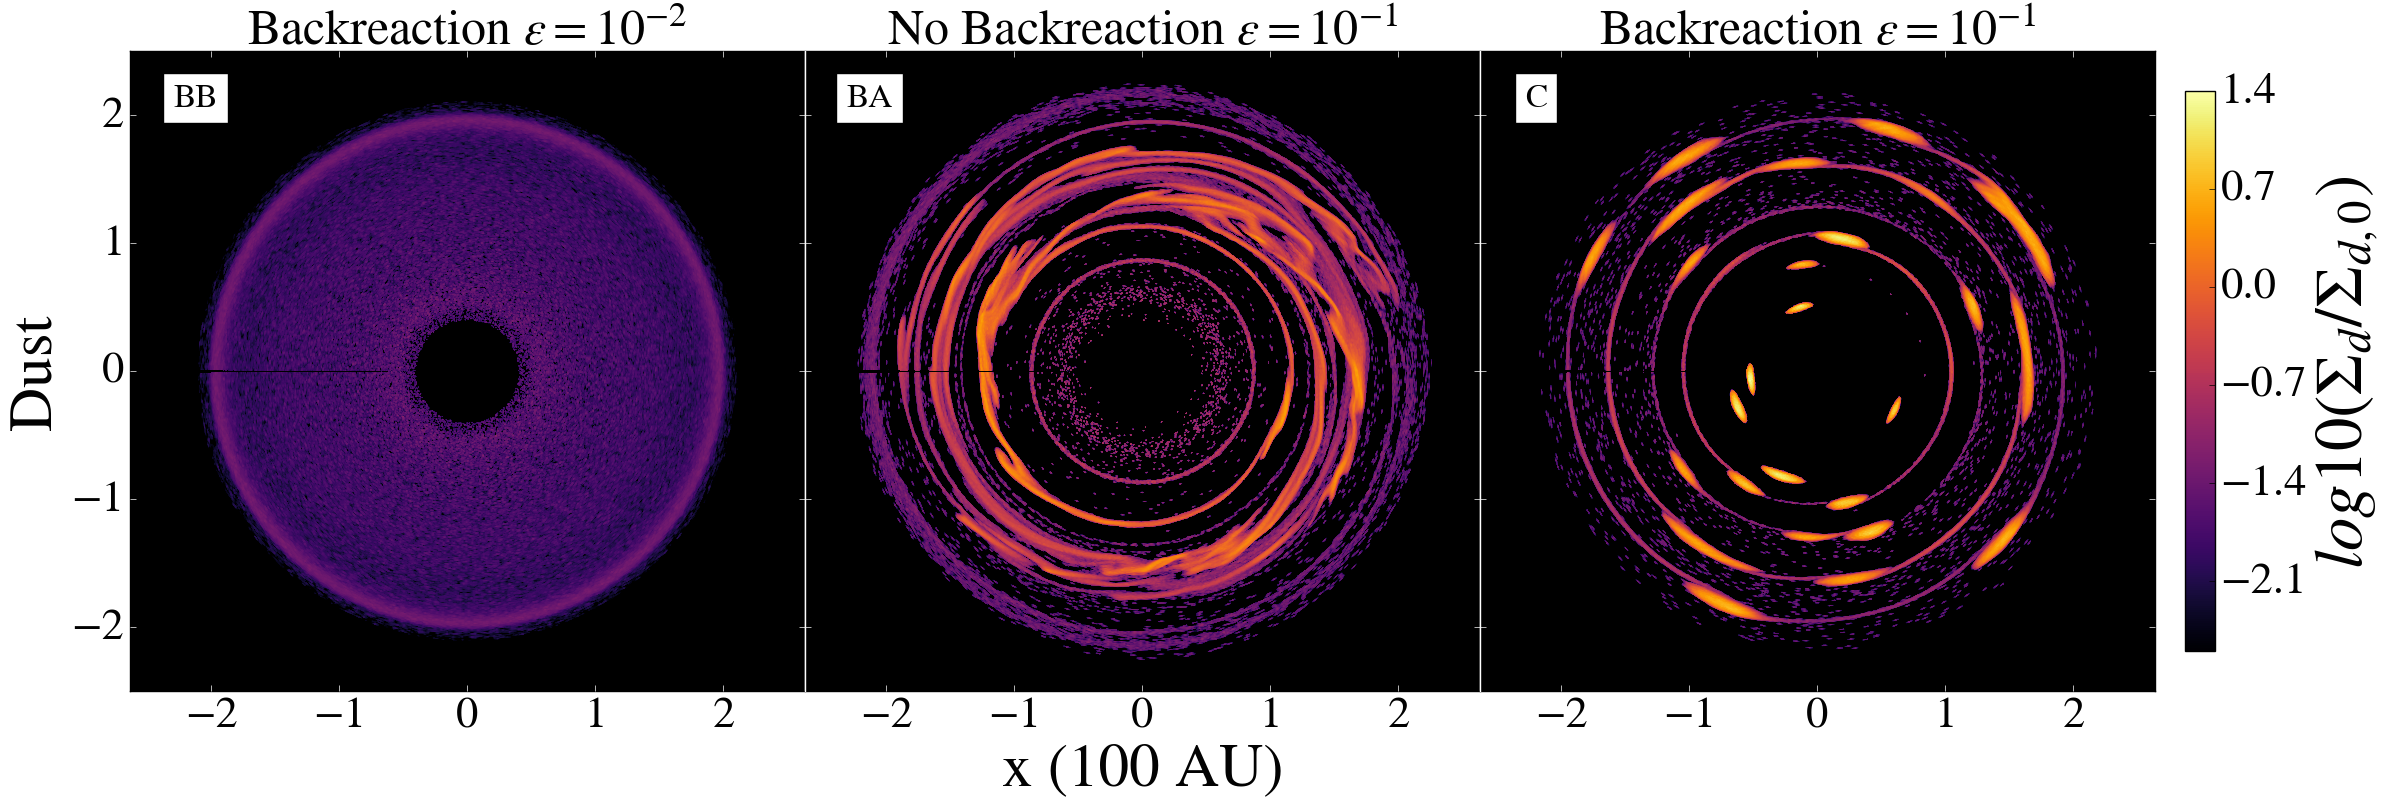
\includegraphics{./05_10-1_10-2_bkrx_nobkrx_dust.png}}
    \resizebox{0.8\textwidth}{!}{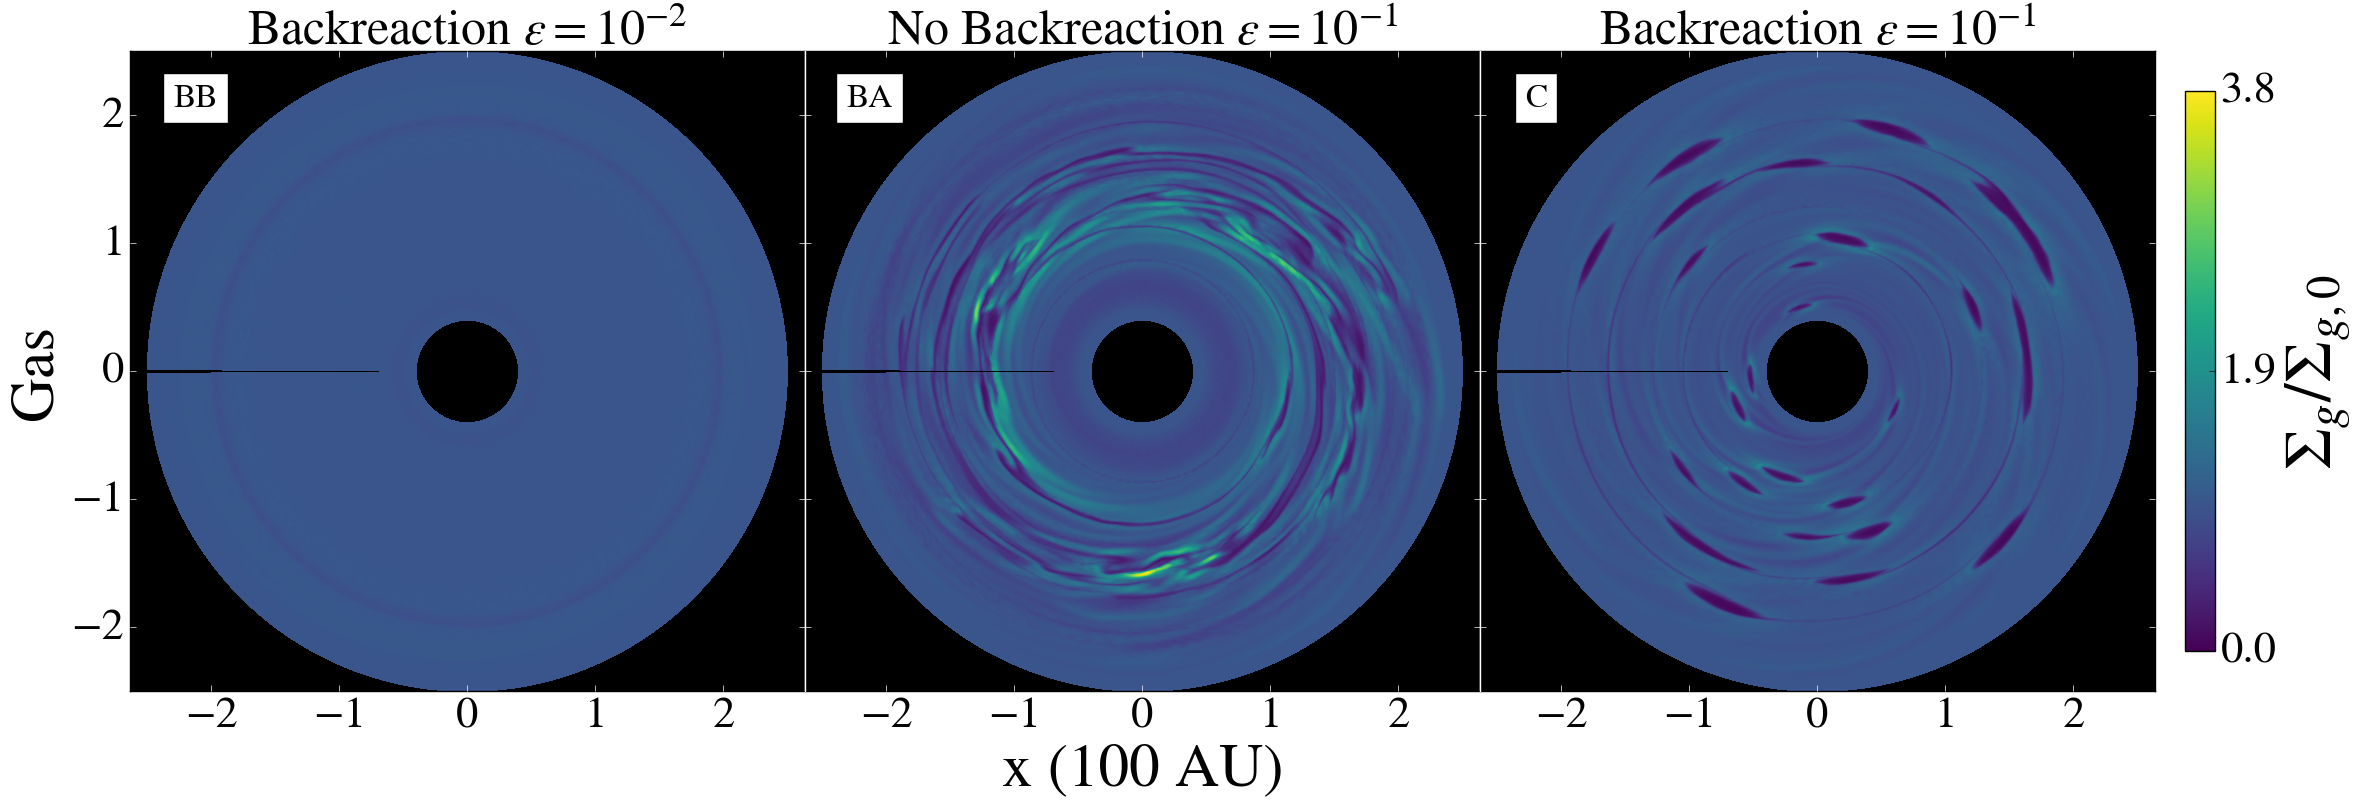
\includegraphics{./05_10-1_10-2_bkrx_nobkrx_gas.png}}
  \end{center}
  \caption{A comparison for the effect with and without backreaction for two dust-to-gas ratios. The two ratios are \
    $\varepsilon=0.1$ and $10^{-2}$. The case with lower dust-to-gas ratio does not yield enough photoelectric heating t\
    o form structures, so the effect of the backreaction being turned off does not change the results.}
  \label{fig:bkrk_comp_two_epsi}
\end{figure}


\begin{figure}
  \begin{center}
    \resizebox{0.6\columnwidth}{!}{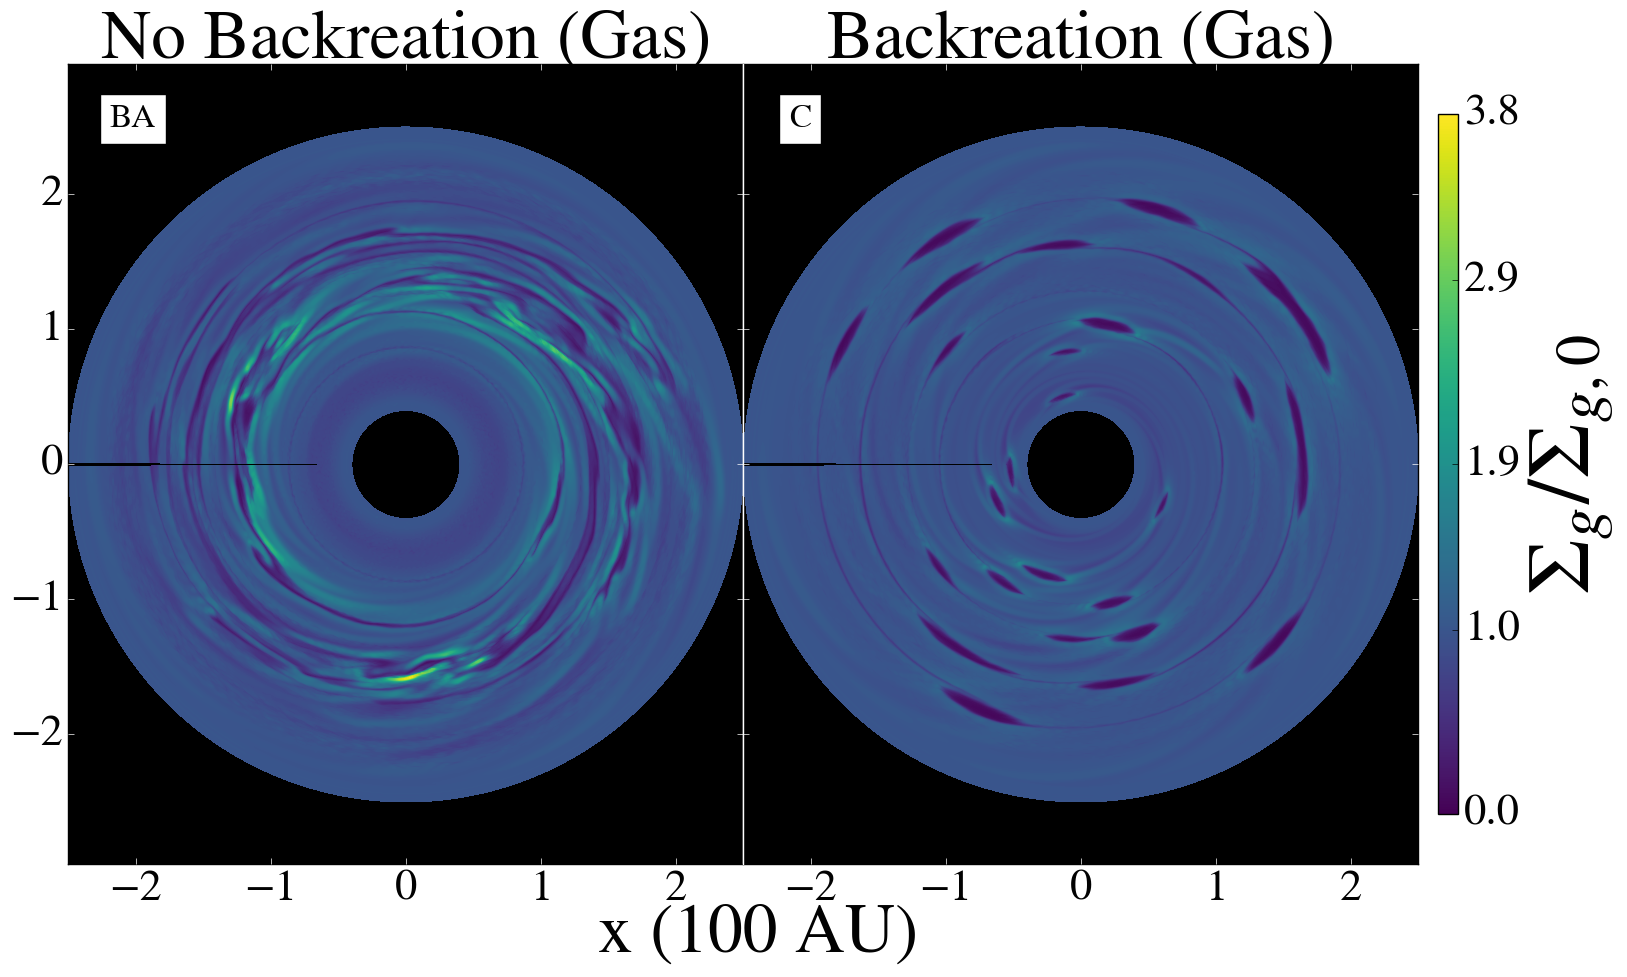
\includegraphics{./05_10-1_comp_bkrx_gas.png}}
    \resizebox{0.6\columnwidth}{!}{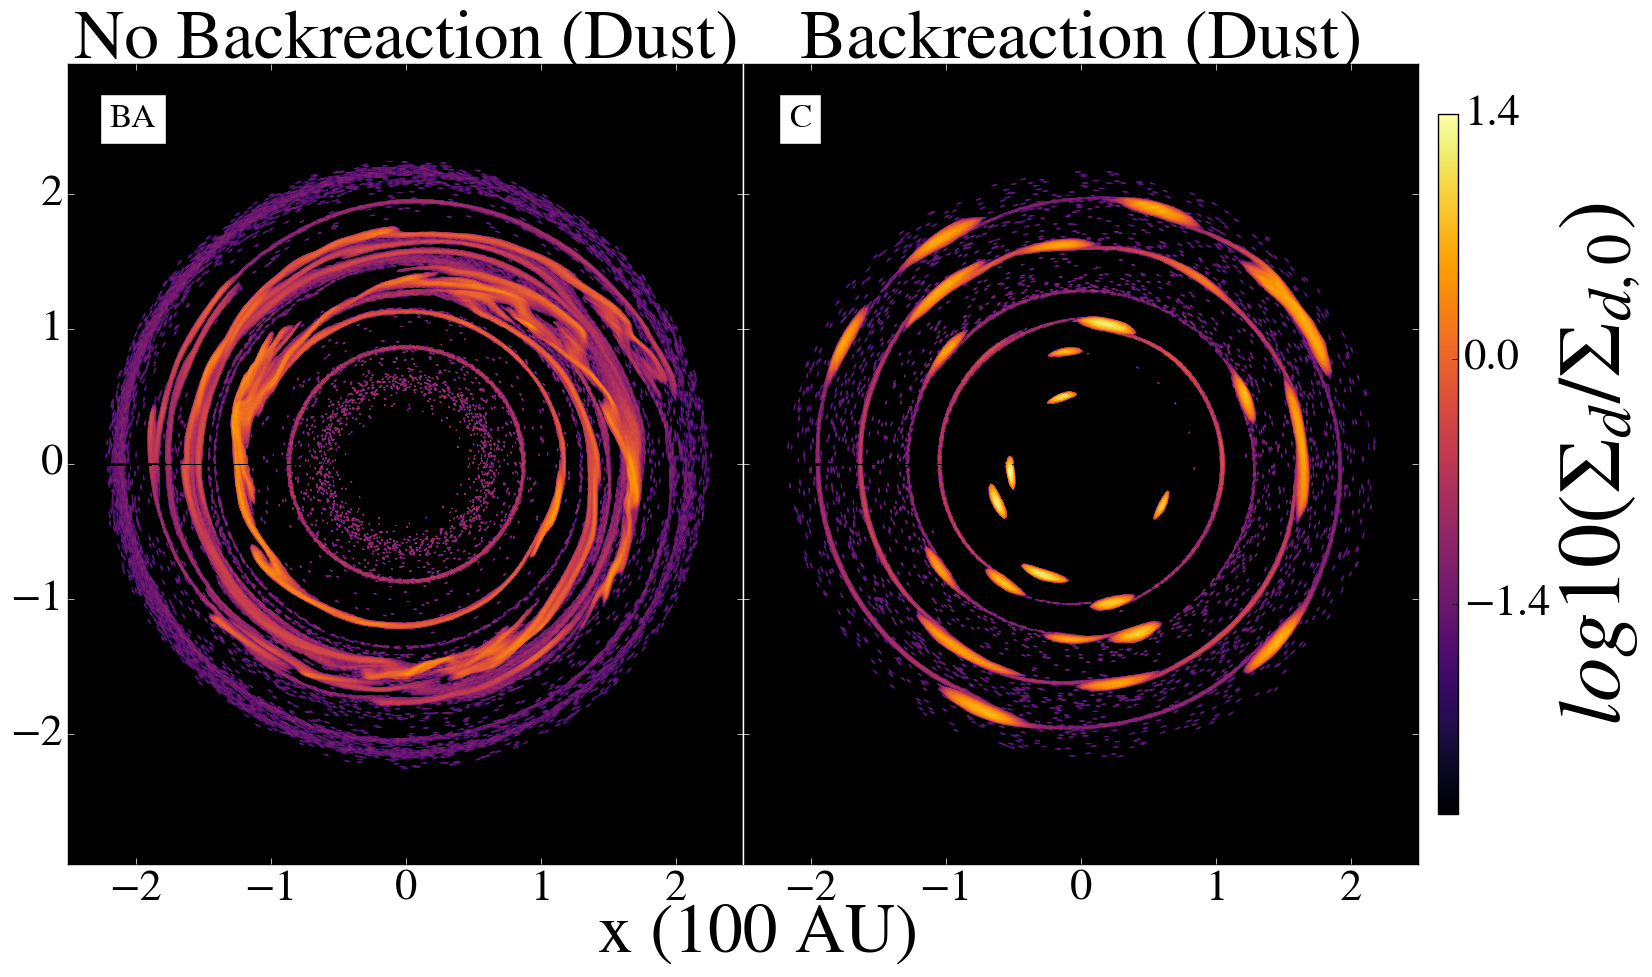
\includegraphics{./05_10-1_comp_bkrx_dust.png}}
  \end{center}
  \caption{A comparison with backreaction active and inactive for a
    disk of $\varepsilon=10^{-1}$ and $h=0.05$. We see that the
    backreaction confines the dust into shapely and organized
    structures.}
  \label{fig:bkrk_comp}
\end{figure}  

In \Fig{fig:bkrk_comp}, we explore the effect of the dust backreaction for a simulation of $\epsi=0.1$. The upper panel show the gas, while the lower plots show the gas. The panels of the left show runs without backreaction, and those on the right show runs with backreaction. We see that the backreaction confines the dust into shapely and organized structures. The run without the backreaction shows spiral features and accumulation at larger distances from the disk, to a lesser degree than in the run for $\epsi=1$ in \textbf{LK13}. We expect that for lower dust-to-gas ratios the backreaction will be less important and. The conclusion is that well-organized PEI structures should be expected only in disks with high dust-to-gas ratio, higher than primordial.

Runs I and J show a disk with PEI and a planet of $q=10^{-3}$ and $q=10^{-4}$, respectively. The more massive pertuber carves out a larger gap in the dust. Comparing run J to run H, we see no discernable differences. This echoes our previous conclusion that only planets that carve substantials caps can be disentangled from the effect of the PEI. For the gas in \Fig{fig:eps1dustgas}, we see similar results to \Fig{fig:eps01dustgas}. Runs I \& J, which include a planet and PEI, show one important difference. The Lindblad spiral of the Neptune analog, which was diminished in run E ($\epsi=0.1$), has all but disappeared in run J ($\epsi=1$), washed out by the stronger effect of the PEI. The Jupiter-mass planet in run I is still visible. showing a gap and the Lindblad spiral.


\Fig{fig:eps1dustprofile} is the same as \Fig{fig:eps01dustprofile}, but now for a dust-to-gas ratio equal to unity. For the Jupiter-mass planet the dust averages are shown on the left-hand side. The dashed red line and the solid black line both contain a planet, and they show a depletion of dust in the vicinity of the planet at r=1. The solid blue line is for a simulation with only the photoelectric instability. The Neptune case is plotted on the right, with the solid black and red line containing a planet. The pure instability, in the blue, coincides almost exactly with the run incliding the instability and a planet. Where they differ is in a park near the planet, inside of the gap. In this case, it can be argued, that with a very accurate observation we should be able to disentangle this planet from the instability. Therefore, it would be a much arduous task in accuracy, to be able to detect such small differences in the observations. 

\section{Dependence on Thermal Mass}

Our results depend on the ability of the planet to carve a gap, the parameter that controls whether this happens or not is dependent not on the mass of the planet, but the thermal mass. The thermal mass is that for which the Hill radius of the planet equals the scale height of the disk.

\beq
q_{\rm th} = 3 h^3
\eeq

For $h=0.05$, a Jupiter-mass planet is equivalent to $q=8q_{\rm th}/3\approx 2.7 q_{\rm th}$ and the Neptune-mass planet to $\approx 0.27q_{\rm th}$.

Increasing the aspect ratio $h$ by a factor 2 (to $h=0.1$) increases
the thermal mass by a factor 8. The Jupiter-mass planet
should become equivalent to $q_{\rm th}/3$, roughly equivalent to the
Neptune-mass planet in the $h=0.05$ case.

We have found the condition that disentangles the carving of a gap from the
structures created from the photoelectric instability.
We take the radius of the dust gap and the frequency of the photoelectric
instability to be $r_{gap}^{(d)}$ and $\lambda_{\rm PEI}$, respectively.
In order for the two processes to be differentiated, we must have that
$r_{gap}^{(d)} > \lambda_{\rm PEI}$. In this case, the gap is large enough
that peaks caused by the instability are within the gap, as is seen in
\Fig{fig:fig_1drad_avg_h01} for the Jupiter case. Comparing this to the
Neptune case in the same figure $r_{gap}^{(d)} \approx \lambda_{\rm PEI}$,
showing no concrete difference between the PEI and combined case.

In the next subsections, we explore the role of temperature.

\section{Disk with $\epsi=1$ and $H=0.1$}

\begin{figure}
  \begin{center}
    \resizebox{.8\textwidth}{!}{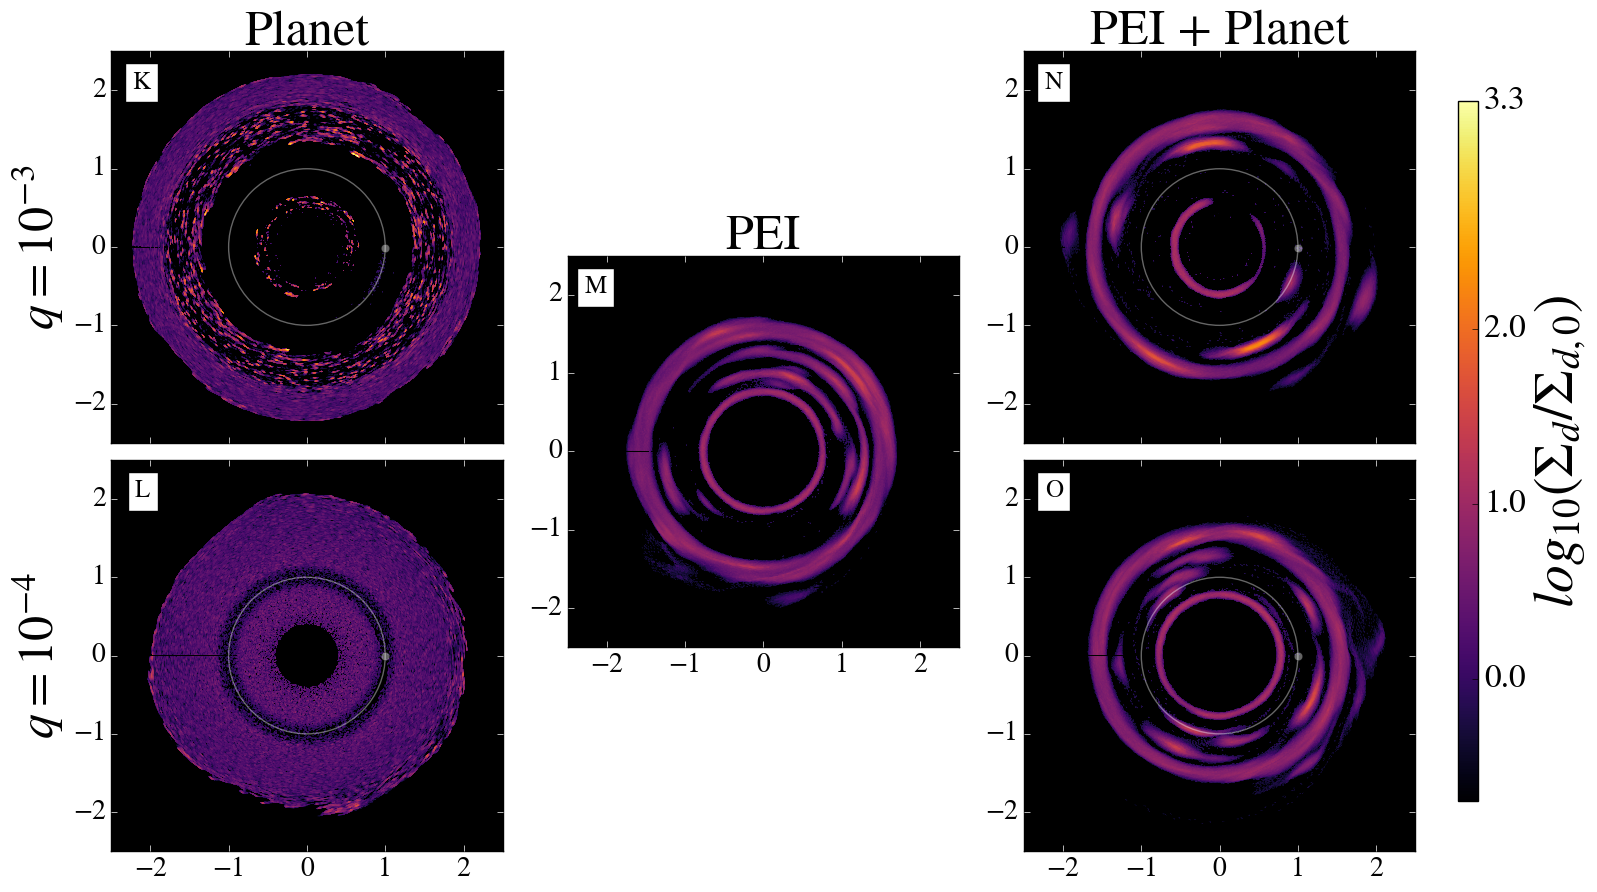
\includegraphics{./1_10-0_dust_global.png}}
    \resizebox{.8\textwidth}{!}{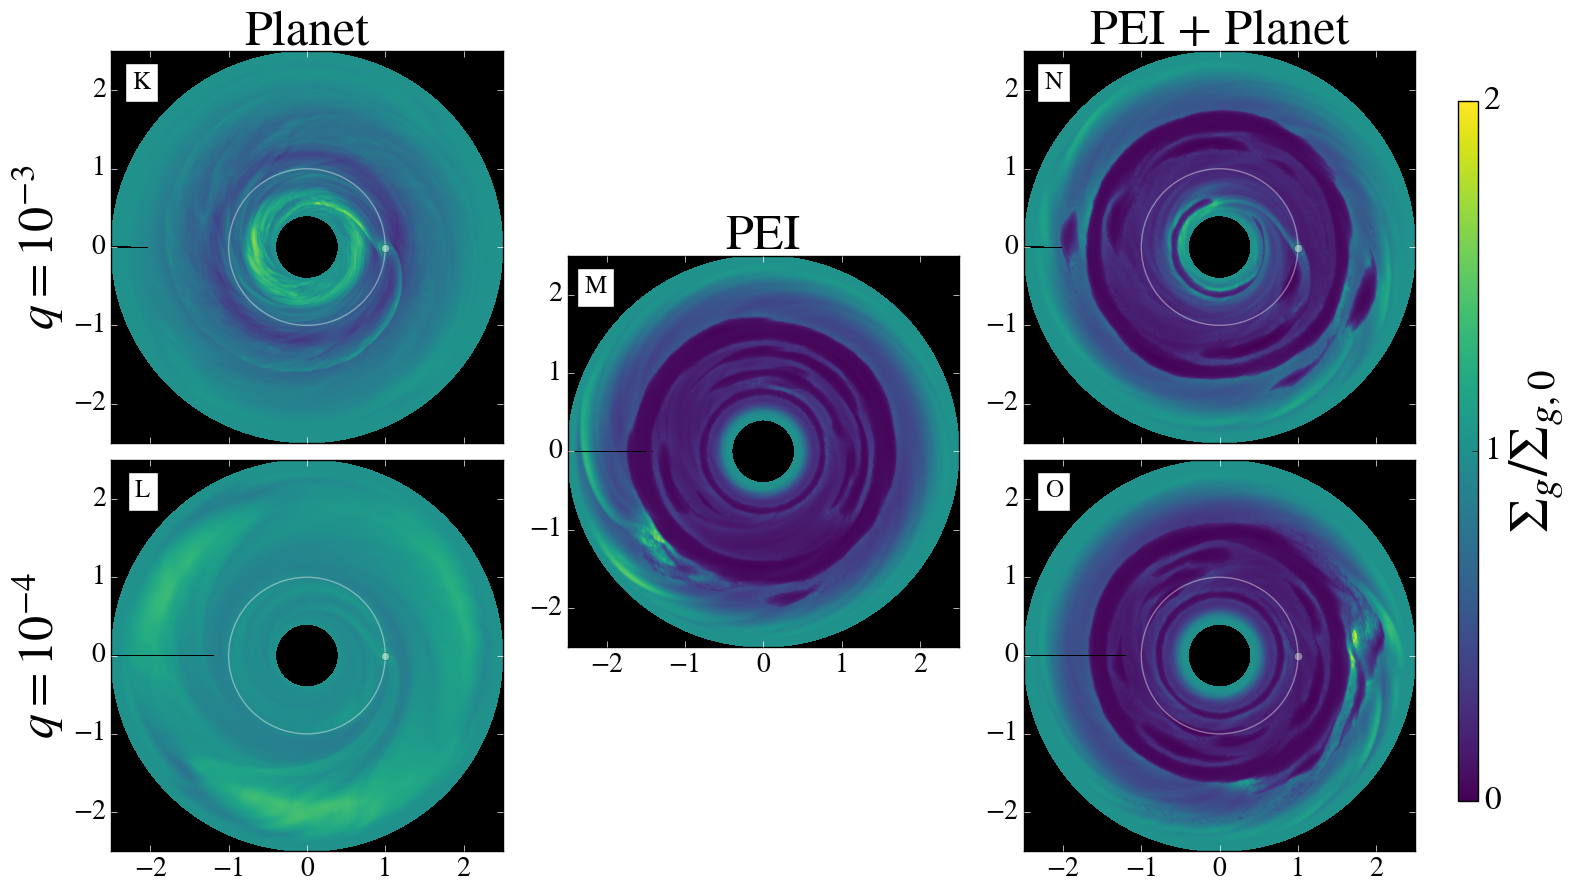
\includegraphics{./1_10-0_gas_global.png}}
  \end{center}
  \caption{Same as \ref{fig:eps1dustgas}, but for $h=0.1$. For the dust
    plots we see the typical clearing out of dust, with the
    Jupiter mass carving a larger gap. The instability case now shows
    only a few arcs and one large diameter ring on the outer edges of
    the disk. The combined case shows the large disk at the outer
    boundaries with some added features. Again the Jupiter-mass planet
    pushes grains away from its gap; and the Neptune-mass planet does
    not generate structures easily distinguishable from the PEI
    alone. With this higher temperature, the Neptune-mass planet does
    not carve a partial gap in the gas, as expected from its lower thermal mass.
    Run L shows an asymmetry in the outer edge of the dust distribution.
    The gas plot reveals that these asymmetries are caused by vortices, in a
    prominent $m=3$ mode. These vortices were generated by Rossby wave instability,
    effected by the backreaction of the dragforce as the dust front drifts inwards.}
  \label{fig:h01dustgas}
  \end{figure} 

\Fig{fig:h01dustgas} shows dust and gas for a disk with aspect ratio of $h=0.1$. The top panel show the dust and the bottom show the gas. The Jupiter-mass planet now has a thermal mass of 0.33, and the Neptune-mass has a thermal mass of 0.03. The Neptune analog does not carve a large enough gap, remaining deeply embedded. The Juper analog als carves a narrower gap, as expected from its thermal mass being lower than 1.

The dust panel of run L deviates from the symmetrical as well as an enhanced dust drift when compared to the Jupiter case in run K. All parameters are equal except for the planet mass. Examining the gas plots, we see prominent strucutures at r=2, somewhat resembling vortices, however these structures are not trapping dust. This only happens if the structures are being triggered after dust has drifted inwards. Indeed, looking at the dust plots, we see that the dust has drifted inward past the location of the vortices.

It is curious that this phenomenon is happening at the outer edges, but since it is not present in the Jupiter case, we can rule out a boundary condition. Instead, we conjecture that we are seeing the Rossby Wave Instability being triggired by the dust drift at this high dust-to-gas ratio. As the dust drifts, it creates a sharp discontinuity. At this dust-to-gas ratio, the backreaction from the gas drag is important dynamically, causing the gas to have differential rotational velocities immediately inside and outside of the dust front. This difference eventually becomes important enough to trigger the RWI. In this case, the dust front is artificial, since we are not replenishing dust particles from the outer boundary. However, there are models where this discontinuity exists, such as in the birth-ring model. In these disks, with a high dust-to-gas ratio, we predict that the RWI should be triggered in the gas. If the vortices disrupt the grains, as in our model, the birth ring will also become eccentric.

The Jupiter-mass planet does not show the same phenomenon due to the reduced dust drift, causing the dust front to remain at the boundary, where the conditions are driven back to initial conditions. We propose that for the $h=0.05$ case this should still be noticed, but the dust has not drifted far enough inwards for the dust front to be resolved outside of the boundary condition. The dust drift is proportional to the sub-Keplerian reduction parameter $\ni$, which is proportional to $h^2$. Increasing h by a factor of 2, increases the drifting time by a factor of 4, making the effect more noticeable.

Run M shows a simulation with PEI and no planet. The simulation contains a smaller number of arcs and more rings when compared to the $h=0.05$ case, the structures are also thicker with a higher value of $H$. The gas disk is empty in the center, due to the increased heating. The gas expands due to the higher temperature, thinning it out. At the boundaries it retains the high initial values due to our boundary that drives values to their original value.

The combined case of a planet and PEI, shown in runs N and O, show rings and arcs as well. Run N, with a larger planet shows a larger gap, with dust depletion in the immediate area. Run O, for a Neptune analog, shows various arcs and a non-discernable gap in the dust.

\section{Disk with $\epsi=1$ and $H=0.2$}

\begin{figure}
  \begin{center}
    \resizebox{.8\textwidth}{!}{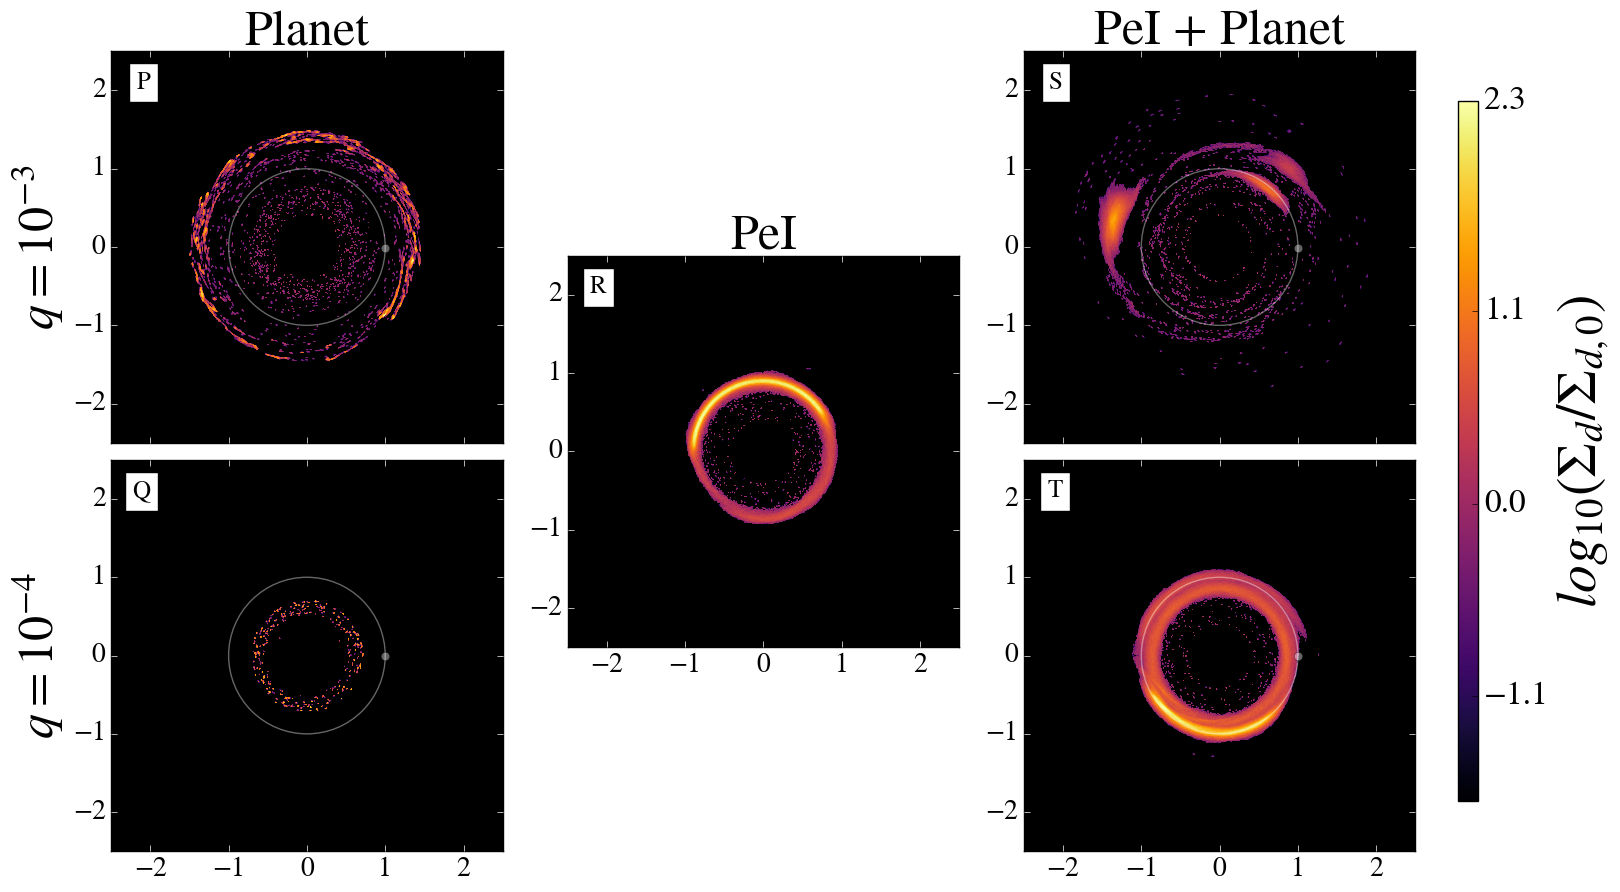
\includegraphics{./2_10-0_dust_global.png}}
    \resizebox{.8\textwidth}{!}{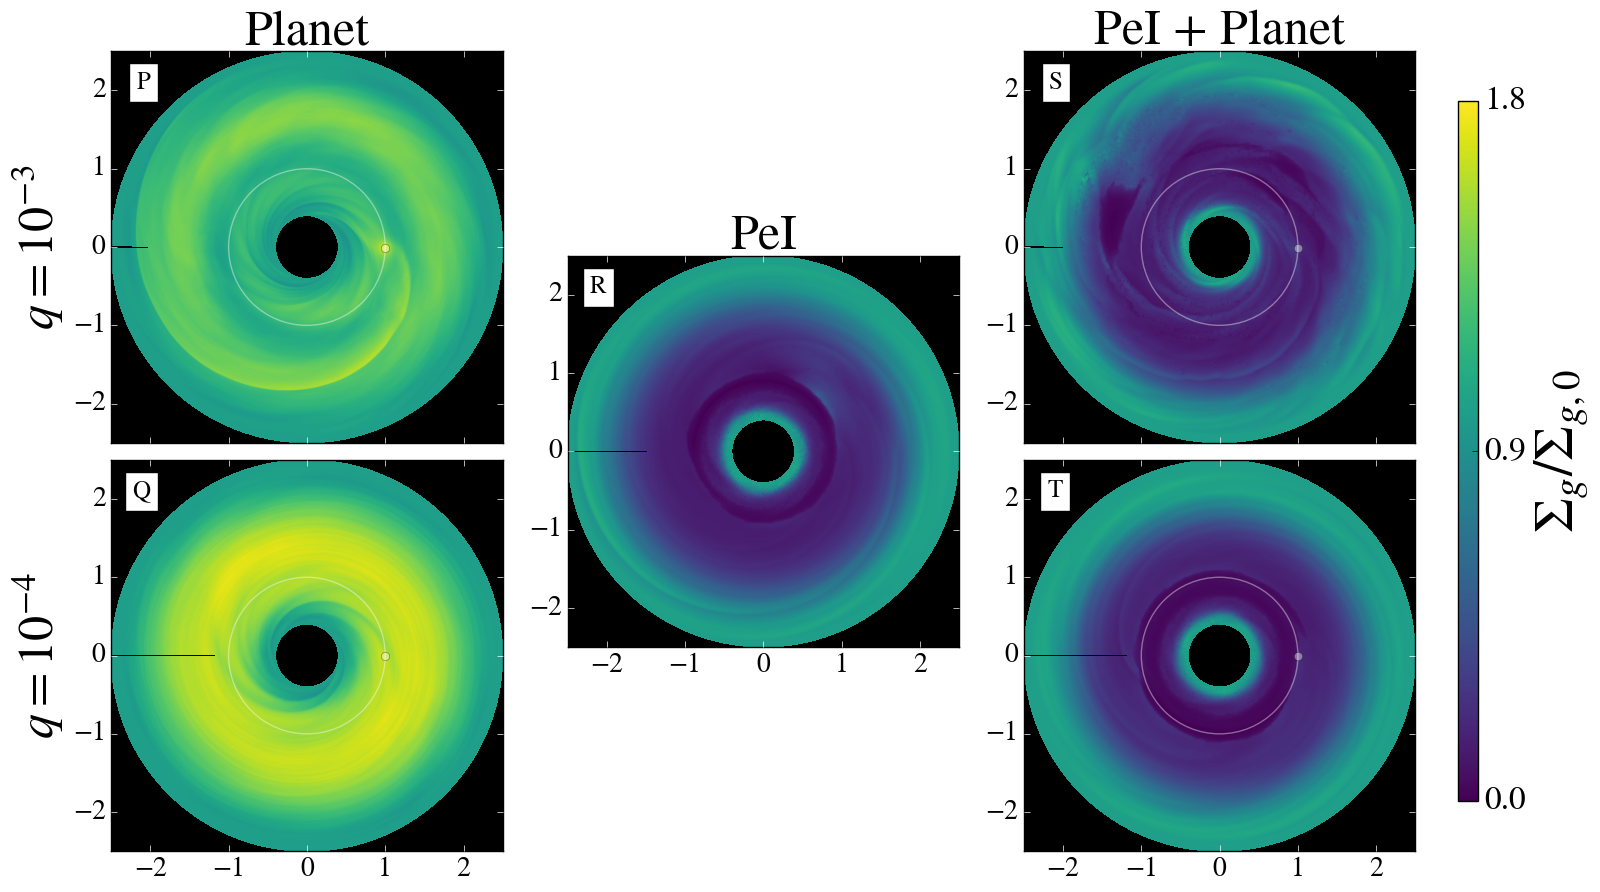
\includegraphics{./2_10-0_gas_global.png}}
  \end{center}
  \caption{Similar to \fig{fig:eps10dustgas}, but for $h=0.2$. In this hot disk, neither of the planets is massive en\
    ough
    to carve a deep gas gap. For the Jupiter case a gap is carved in the dust, but for the Neptune case
    the dust streams past the planet's orbit (left plots). This is because in this
    hot disk the drift time past the planet's corotational region
    is faster than a planetary orbit. For the Neptune case, these times
    are comparable (see \sect{sect:eps1h02}) and the dust can stream
    past the planet. The Jupiter-mass planet, with a larger
    corotational region, will be able to scatter the grains and carve
    a deep dust gap. The combined effect of a planet and the instability is barely
    distinguishable from purely PEI in this hotter disk, mostly
    because a gap is not carved and most of the dust has rapidly
    drifted inwards.}
  \label{fig:h02dustgas}
\end{figure}


Finally we considered a disk with a scale height of $h=0.2$, which is on the hotter side for primordial disks, but typical for debris disks with gas, including $\beta$ Pictoris. We plot in \Fig{fig:h02dustgas}, on the top panel, the dust structures, and the gas structures in the lower panel. For the Jupiter case, in the upper left, we see a gap being carved in the dust. For the Neptune case, however, we only see a small ring in the inner part of the planet, and nothing outward. This means that the dust is drifting much faster for the Neptune case than the Jupiter case. This effect is due to two mechanisms. Firstlu, the Jupiter-mass planet, has a thermal mass of 0.04, so it carves a very narrow gap. The less massive planet has a reduced thermal mass of 0.004, so it is unable to open a gap. The high density caused by the Jupiter-mass planet carving a gap, traps the grains, stopping them from moving father inward. For the Neptune case, they stream past the planet orbit, and are only caught inside the planet, due to the \textbf{dust piling up.}

The dust grains are able to stream past the planet, somehow bypassing the dust filtering that planets usually achieve. The seems to happen because the drift speed of the grains is faster than the planet orbiting. We can compare the time it takes a grain to drift past the corotational region, and the orbital peroid of the planet. The equation for that is:

\beq
\Theta  = \frac{t_{\rm drift}}{t_{\rm orb}}
\eeq

If $\Theta>1$, then the drifting is slow and the planet is able to hinder the planets crossing into the inner part of the disk. On the other hand, if $\Theta<1$ then the planet is too slow and the grains can begin drifting past it. We consider the drift velocity of a particle from Youdin (2010):

\beq
v_r = -\frac{2\St\,\eta\,v_k}{1+\St^2},
\eeq

\noindent where $v_k=\varOmega_k r$ is the Keplerian velocity and

\beq
\eta \equiv = -\frac{1}{2\rho\varOmega^2r}\frac{\partial p}{\partial r}
\eeq

\noindent is the sub-Keplerian parameter. The time it takes to drift is $v_r/2x_s$ where $x_s$ is the
half-width of the corotational region, given by \textbf{PaardekooperPapaloizu09}

\beq
x_s^2 = 1.68 r_p^2 \frac{q}{h}
\eeq

\noindent and $r_p$ the planet's location. Solving for $\Theta$,

\beqn
\Theta &=& \frac{\varOmega  x_s}{\pi v_r }\\
&\approx&0.4 \ q^{1/2} h^{-5/2} \chi^{-1} \St^{-1} \left(1+\St^2\right)
\eeqn

\noindent where $\chi=\alpha+\beta$ with $\alpha=-\partial\ln \rho/\partial\ln r$ and
$\beta=-\partial\ln T/\partial\ln r$.  For $q=10^{-4}$, $h=0.2$, $\St=1$
and considering $\alpha+\beta=1$, we get $\Theta=0.5$. For the
Jupiter-mass planet, $\Theta=1.4$. Thus, it is possible that
in the Neptune-mass case the $\St=1$ grains can drift past the corotational
region in this hot disk. However for the Jupiter-mass planet, having a larger corotational region,
it should be able to disperse the dust grains and carve a discernable gap.

In the simulation with photoelectric instability (run R), we see a
much denser ring of dust in the center of the disk. The combined case
of instability plus planet (runs S and T) are shown in the plots in
the right hand side. For the massive planet (run S) the main differences are
that the grains, instead of being scattered roughly uniformly as in
run P, now concentrates in arcs. Additionally, an arc coinciding with
the location of the Lagrange point L5 is prominent. The lower mass
planet (run T) seems indistinguishable from the pure instability case
(run R), having a similar distribution of dust concentration.

The behavior of the gas (lower plots) resembles the case for
$h=0.1$. The gas density is much lower throughout the disk
due to the enhanced photoelectric heating, being driven back to the
initial value at the boundaries. A spiral is barely discernible for
Jupiter-mass planet. No clear distinction is present for the lower
mass planet.

\section{Conclusions}

Here we have considered for the first time, disk-planet interactions with the presence of the photoelectric instability. We also study for the first time, planet-disk interactions for disk with a dust to gas ratio of unity. The gap walls, acting as dust traps, are places where deviation occurs. At global dust-to-gas ratio, $\epsi=10^{-2}$, the effect starts becoming noticeable with a small reduction in the height of the gap wall. For $\epsi=10^{-1}$, and $\epsi=1$m the gap wall becomes significantly shorter as the local dust enhacement reaches above unity. This result does not depend on the photoelectric instability and applies to optically thick disks, such as primordial and gas-rich transition disks.

Our simulations show that when we include the photoelectric instability, structures produced by low-mass planets are not easily discerned, from those incited by the pure instability. A large gap being carved, and the presence of a presence of a spiral are still the tell-tale signatures of planets, as is usually the case for conventional transition disks. The clearest sign of a planet is the radial clearing in the PEI-induced structures, wider than the typical periodicity of the instability. That is, we can distinguish a planet amid photoelectric instability structures if the planet carves a dust gap larger than the wavelength of the photoelectric instability. Quantitatively, we can state that the criterion for a planet to be distiguishable from the PEI is such that, $\Delta r^{(d)}_{\rm gap} > \lambda_{\rm PEI}$, where $\Delta r^{(d)}_{\rm gap}$ is the radial width of the dust gap and $\lambda_{\rm PEI}$ the wavelength of the instability. The quantity $\Delta r^{(d)}_{\rm gap}$ is the simpler one to quantify. The boundary of the dust gap is located at the edge of the gas gap, that functions as a dust trap. As for $\lambda_{\rm PEI}$, linear instability analysis predicts growth even for large wavenumbers, $k\rightarrow\infty$ \textbf{LyraKuchner13}. Regularizing with viscosity produces the most unstable wavelength of the order of the scale of viscous dissipation, which is very small in primordial and transitional disks, but of order AU in late transition and debris disks. Yet, a 3D run in \textbf{LyraKuchner13} shows ring spacing of $\approx 0.1H$ for a simulation with grid resolution $dx=H/256 \approx 0.004$, i.e., $\lambda_{\rm PEI}/dx \approx 25$, and thus far from the viscous range. A specific prediction for $\lambda_{\rm PEI}$ is still lacking in the literature, a situation that is compounded by the fact that the PEI also exists in the nonlinear regime.

We have also shown that the PEI leads to well-defined sharp strucures, but only for high dust-to-gas ratios, because of the pivolal role of the drag force backreaction in capturing the dust. Simulations without backreaction, or with too little dust, $\epsi \approx 10^{-1}$, easily break into spiral structures and turbulence. We conclude that well-organized PEI structures should be expected only in disks with dust-to-gas ratios higher than primordial \textbf{what is primordial?}

Finally, incomplete arcs are not produced in simulations with planets alone; they require the photoelectric instability in order to form. However, we do not consider situations with self-gravity, which is thought to be a component in a possible mechanism to maintain incomplete arcs, mainly in Neptune's rings (\textbf{NamouniProco02; Tsui18}). Although this is unlikely in the csae of debris disks, of very low mass, to produce a noticeable effect.

The models of \textbf{Richert+18} show that radiation pressure can have a significant effect on the global dust distributions of optically thin disks. The models presented in \textbf{Section 3} are most applicable to optically thin disks around low mass stars (spectral typess K \& M) and white dwarfs, since their low luminosities supply a small amount of radiation pressure even on small particles. THese particles are usually well-coupled with ($\tau\Omega = 1$). Therefore, more luminous stars will exert a larger radiation pressure that will likely cause the disk morphology to deviate from our models. Our models, and those of \textbf{Richert+18}, show that radiation pressure, massive planets, and the photoelectric instability can all have an important role in shaping the morphology in optically thin disks. Therefore, future research should extensively explore the combination of these and other effects. In particular, it should be noted that the MRI could be a potentially important process \textbf{KralLatter16}, which has to this point not been explored. 

\chapter{Application to the Observations: HD141569A}

Now that we have all this theory and results, we want to apply them to current observations, to test if they are in line with real-life physics. The one disk that we chose is HD141569A, which is pictured in \textbf{insert HD picture here}. This is a good candidate to be exhibiting the PEI due to its age, its dust-to-gas ratio and previous observations. Looking at previous observations we see that the disk shows the same axisymmetric structures, such at the arcs, rings, and gaps that are pertinent to the PEI. Looking at the next figure, we see that observations and different wavelengths show the same structures as a simulations from \textbf{Lyra \& Kuchner 2013, insert figure of observations and simulation.}



In order to do that, we have to employ another type of code. This is a radiative transfer code called RADMC3D. RADMC3D takes the information from our code, mainly from the dust density in the disk. The code does photon interaction within the disk for certain wavelenghts. From this information is creates an image at the different wavelengths that would reflect what the disk would look like from an observation.


\clearpage
\addcontentsline{toc}{section}{\hspace{-19pt} References}
\singlespacing
\begin{thebibliography}{}

\bibitem{alma-et-al_2015}
ALMA Partnership et al. 2015, ApJL, volume 808, issue 1, article id L3, 10 pp.

\bibitem{andrews-et-al_2016}
Sean M. Andrews et al. 2016, ApJL, 820, L40, 5

\bibitem{armitage_2011}
Philip J. Armitage 2011, ARA\& A, 49, 195-236

\bibitem{baehr-klahr-kratter_2017}
Hans Baehr, Hubert Klahr, \& Kaitlin M. Kratter 2017, ApJ, 848:40, 10

\bibitem{TPS}
Cl\'ement Baruteau. Toward predictive scenarios of planetary migration. Astrophysics [astroph].
Observatoire de Paris, 2008. English. $<$tel-00334456$>$

\bibitem{bate_2018}
Matthew R. Bate 2018, MNRAS, 475, 5618-5658

\bibitem{boehler-et-al_2018}
Y. Boehler et al. 2018, ApJL, 853, 162, 13

\bibitem{brandenburg-dobler_2010}
Axel Brandenburg \& Wolfgang Dobler 2010, Astrophysics Source Code Library, ascl:1010.060

\bibitem{choudhuri_1998}
Arnab Rai Choudhuri 1998, $The Physics of Fluids and Plasmas: An Introduction for Astrophysicists$ (Cambridge University Press), 31-83

\bibitem{elsasser-staude_1978}
H. Elsasser \& H.J. Staude 1978, A\&A, 70, L3-L6

\bibitem{gammie_2001}
Charles F. Gammie 2001, ApJ, 553, 174-183

\bibitem{kratter-lodato_2016}
Kaitlin Kratter \& Giuseppe Lodato 2016, ARA\& A, 54, 271–311

\bibitem{lin-shu_1964}
C.C. Lin \& Frank H. Shu 1964, AJ, 140, 646

\bibitem{meru-bate_2012}
Farzana Meru \& Matther R. Bate, 2012, MNRAS, 427, 2022–2046

\bibitem{meru-et-al_2017}
Farzana Meru et al. 2017, ApJL, 839, L24, 6pp

\bibitem{paardekooper_2012}
Paardekooper 2012, MNRAS, 421, 3286–3299

\bibitem{perez-et-al_2016}
Laura M. Perez 2016, Science, 353, 6307, 1519-1521

\bibitem{rice-lodato-armitage_2005}
W. K. M. Rice, G. Lodato, \& P.J. Armitage 2005, MNRAS, 364, L56-L60

\bibitem{rucinski_1985}
S.M Rucinski 1985, AJ, 90, 11

\bibitem{smith-terrile_1984}
Bedford A. Smith \& Richard J. Terrile 1984, Science, 226, 4681, 1421-1424.

\bibitem{toomre_1964}
Alar Toomre 1964, ApJ, 139, 4, 1217-1238

\bibitem{watson-et-al_2007}
Alan M. Watson, Karl R. Stapelfeldt, Kenneth Wood, \& Francois Menard 2007, Protostars and Planets V, University of Arizona Press, 951,523-538

\end{thebibliography}

\end{document}
